\documentclass{article}

\usepackage{amsmath, amssymb}
\usepackage{mathtools}
\usepackage{graphicx}
\usepackage{hyperref}
\hypersetup {
    colorlinks = true, %
    linkcolor = blue %
}

\newcommand{\dx}{\, dx}
\newcommand{\dy}{\, dy}
\newcommand{\dA}{\, dA}
\newcommand{\du}{\, du}
\newcommand{\dw}{\, dw}

\title{Interesting Examples in Undergraduate Mathematics}
\author{Matthew McGonagle}

\begin{document}

\maketitle

\tableofcontents

\section{Introduction}

The purpose of these notes is examples in undergraduate mathematics that the author considers to be interesting; this could be from applications or pure mathematical interest. 

\section{Precalculus}
\subsection{Descarte's Method of Tangents}

\subsubsection*{The Setup}

Prior to the differential calculus created by Leibniz and Newton, Descarte invented several methods of 
finding tangent lines to curves that are described by algebraic equations. These methods are purely
algebraic; they don't use either the concept of limits or infinitesimals. A nice reference on these
methods is Suzuki \cite{descarte}. Here we will discuss one of Descarte's simpler methods. As an example,
we will use Descarte's method to find the tangent line to the ellipse \(\{x^2 + 2y^2 = 3\}\) at the
point \((1,1)\).

To begin, let us define the two variable polynomail \(p(x,y) = x^2 + 2y^2 - 3\); we see that our ellipse is
the zero set \(\{p(x,y) = 0\} \).

Next, let us describe all of the non-vertical lines (not necessarily tangent lines) that pass through the 
point \((1,1)\). Consider any line \(y = mx + b\). If this line passes through \((1,1)\), then we have
\(1 = m + b\). So all of these lines are described by \(y = mx + 1 - m\) for different constants \(m\).

Next, let us observe that the interior of the ellipse is the set \(\{p(x,y) < 0\}\) and the exterior
is the set \(\{p(x,y) > 0\}\).
\begin{figure}[h]
\centering
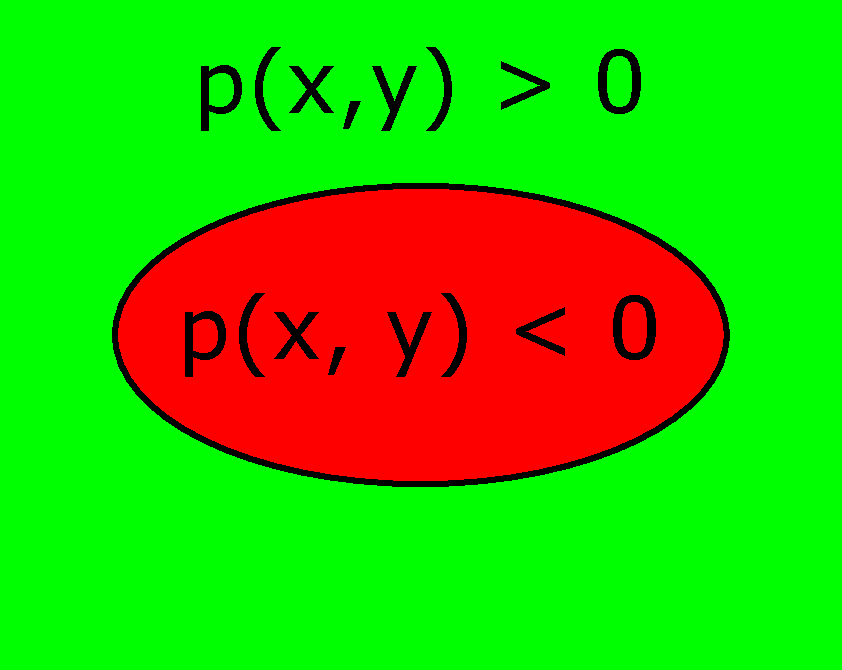
\includegraphics[width=2.5in]{_generated/signPoly.pdf}
\end{figure}

Next, let us see what the sign of \(p(x,y)\) looks like along different lines passing through \((1,1)\). 
When a line passing through \((1,1)\) is not a tangent line, close to \((1,1)\) the line passes through
both the interior and exterior of the ellipse. Therefore, for a non-tangent line, the sign of \(p(x,y)\)
changes. However, a tangent line will remain in the exterior of the ellipse (except at the point \((1,1)\)),
so \(p(x,y)\) will not change sign along the line. Consider the figure below.
\begin{figure}[h]
\centering
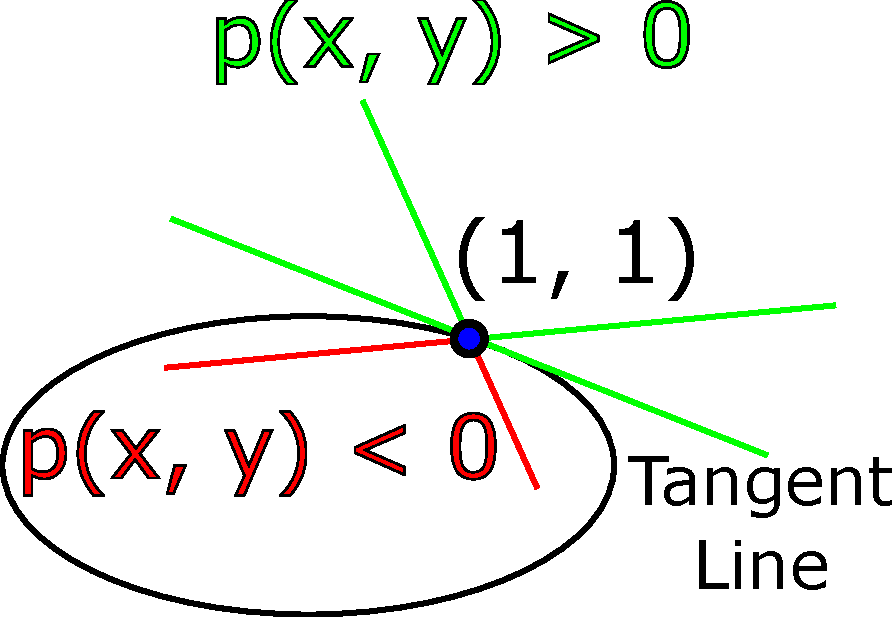
\includegraphics[width=2.5in]{_generated/signTangentLines.pdf}
\end{figure}  

So, given a line \(y = mx + 1 - m\) passing through \((1,1)\), let us compute the value of \(p(x,y\) along
the line. We parameterize this value by \(x\), so we have
\begin{align}
q(x) & \coloneqq p(x, mx + 1 - m), \\
    & = x^2 + 2(mx + 1 - m)^2 - 3, \\
    & = (1 + 2m^2)x^2 + 4(m - m^2) x + 2(1 - m)^2 - 3.
\end{align}

Now, we know that \(q(1) = 0\) since the line must intersect the ellipse at \((1,1)\). Futhermore, from our
argument above, we know that for non-tangent lines \(q(x)\) changes sign at \(x = 1\) and that the tangent
line must NOT change sign at \(q(x) = 1\).

Since the tangent line doesn't change sign, we know that for the correct value of the slope \(m\) for the
tangent line, the polynomial \(q(x)\) has a double root at \(x = 1\). Therefore, for the tangent line,
the polynomial is divisible by \((x - 1)^2 = x^2 - 2x + 1\); that is, after computing the polynomial division
\(\frac{q(x)}{x^2 - 2x + 1}\) we find a remainder of zero.

If we find that there is only one value of \(m\) that gives us a remainder of zero for this polynomial division,
then it must be the slope of the tangent line. Note that for non-tangent lines, we could also have that
\(q(x)\) is divisible by \((x - 1)^2\), since the sign will also change if there is a triple root.

\subsubsection*{The Problem}

Compute the slope of the tangent line \(y = mx + 1 -m\) passing through \((1,1)\) for the ellipse 
\(\{x^2 + 2y^2 = 3\}\) by finding the value of \(m\) for which the polynomial division
\begin{equation}
\frac{(1 + 2m^2)x^2 + 4(m - m^2)x + 2(1 - m)^2 - 3}{x^2 - 2x + 1},
\end{equation}
has vanishing remainder.

\subsubsection*{The Solution}

Let us perform the polynomial division.
\begin{align}
& \frac{(1 + 2m^2)x^2 + 4(m - m^2)x + 2(1 - m)^2 - 3}{x^2 - 2x + 1}, \\
= \, & 1 + 2m^2 + \frac{(2 + 4m^2 + 4m - 4m^2)x - 1 - 2m^2 + 2(1 - m)^2 - 3}{x^2 - 2x + 1}, \\ 
= \, & 1 + 2m^2 + \frac{(2 + 4m)x - 4m - 2 }{x^2 - 2x + 1}.
\end{align}
The degree of the numerator is less than the denominator, so the numerator is the remainder. Therefore,
we must have that \((2 + 4m)x - 4m - 2 = 0\). So the coefficients must vanish and we get
\begin{equation}
\begin{cases}
2 + 4m = 0, \\
-4m - 2 = 0.
\end{cases}
\end{equation}
The system has the unique solution \(m = -1/2\); therefore the slope of the tangent line must be \(m = -1/2\).
So we find the tangent line to be
\begin{equation}
y = -\frac{1}{2}x + \frac{3}{2}.
\end{equation}

\subsection{Cardano's Method of Solving Cubic Equations}

In this section we will look at Cardano's method for solving cubic equations using a specific example. We
will motivate the algebraic manipulations using Cardano's geometric manipulations. For a reference on Cardano's
point of view, see \cite{cardano}. 

\subsubsection*{The Setup}

\newcommand{\boxDim}[3]{{#1} \times {#2} \times {#3}}
Cardano's method is based on geometry. Consider the equation
\begin{equation}
x^3 = 6x^2 + x + 2.
\end{equation}
Cardano considers this as a geometric problem of matching volumes. The left hand side represents
the volume of a cube of side lengths \(x\). Each term on the right hand side represents a specific volume.
So we have

\begin{tabular}{p{0.45\textwidth} | p{0.45\textwidth}}
    Left & Right \\
    \begin{itemize}
    \item Cube with side lengths \(x\).
    \end{itemize} 
    
    &
    \begin{itemize}
    \item Box of dimensions \(\boxDim{6}{x}{x}\). 
    \item Box of dimensions \(\boxDim{1}{1}{x}\).
    \item Cube of side lengths \(2^{1/3}\). 
    \end{itemize} 
\end{tabular}

Now, Cardano's idea is to break up the length \(x\) into two lengths \(a\) and \(b\). That is we, look at
\(x = a + b\).

When we do so, we get

\begin{tabular}{p{0.45\textwidth} | p{0.45\textwidth}}
    Left & Right \\
    \begin{itemize}
    \item Cube of side lengths \(a\).
    \item Cube of side lengths \(b\).
    \item Box of dimensions \(\boxDim{3a}{b}{b}\).
    \item Box of dimensions \(\boxDim{3b}{a}{a}\).
    \end{itemize}
    
    & 
    
    \begin{itemize}
    \item Box of dimensions \(\boxDim{6}{a}{a}\).
    \item Box of dimensions \(\boxDim{6}{b}{b}\).
    \item Box of dimensions \(\boxDim{12}{a}{b}\).
    \item Box of dimensions \(\boxDim{1}{1}{a}\).
    \item Box of dimensions \(\boxDim{1}{1}{b}\).
    \item Cube of side lengths \(2^{1/3}\). 
    \end{itemize}
\end{tabular}

Cardano's idea is to use some or all of the non-cube volumes on the left to cancel problematic terms on the right.
This is done in two stages:
\begin{enumerate}
\item (Depress the Cubic) Divide \(x = a + b\), and use \(a,b\) to remove the second order terms from the equation.
\item Say the new free variable is \(a\), then divide \(a = c + d\) and use \(c,d\) to remove the first order terms. 
\end{enumerate} 
We will look at following these ideas using algebraic manipulation.

\subsubsection*{The Problem}
Use Cardano's ideas to solve 
\begin{equation}
x^3 = 6x^2 + 3x + 2.
\end{equation}

\subsubsection*{The Solution}

We follow the two stages of Cardano.

\begin{enumerate}
\item Fist we depress the cubic. We split \(x = a + b\). So we get
\begin{equation}
a^3 + 3a^2b + 3 ab^2 + b^3 = 6a^2 + 12 ab + 6b^2 + 3a + 3b + 2.
\end{equation}
Now, note that if we fix \(b\) and let \(a\) be a new free variable, then it is possible to eliminate all
terms for \(a^2\). That is we need to find \(b\) such that \(3a^2b = 6a^2\). So we choose \(b = 2\). Then
we get
\begin{equation}
a^3 + 12a + 8 = 24a + 24 + 3a + 8.
\end{equation}
Collecting all non-third order terms to the right, we get
\begin{equation}
a^3 = 15a + 24.
\end{equation}

\item Now we split \(a = c + d\) to get
\begin{equation}
c^3 + 3c^2d + 3cd^2 + d^3 = 15c + 15d + 24. 
\end{equation}
Now, note that to get rid of first order terms and not introduce second order terms, we must use the entirety of the
non-cube terms on the left \(3c^2d + 3cd^2\) and eliminate all of the linear terms on the right \(15c + 15d\).
So we look at the possibilities of matching
\begin{equation}
3c^2d + 3cd^2 = 15(c + d).
\end{equation}
Now, note that \(3c^2d + 3cd^2 = 3cd(c + d)\). So, we are lead to \(3cd = 15\). Now after eliminating the matching, we
have the following system
\begin{equation}
\begin{cases}
c^3 + d^3 = 24, \\
cd = 5.
\end{cases}
\end{equation}

From this, we get that
\begin{equation}
125 + d^6 = 24d^3.
\end{equation}
This is quadratic in \(d^3\), so we may solve for \(d^3\) using the quadratic formula. We get
\begin{align}
d^3 & = \frac{24 \pm \sqrt{24^2 - 4 * 125}}{2}, \\ 
& = 12 \pm \sqrt{144 - 125}, \\ 
& = 12 \pm \sqrt{19}.
\end{align} 
Before, we continue, note that
\begin{align}
\frac{1}{12 + \sqrt{19}} & = \frac{12 - \sqrt{19}}{144 - 19}, \\
    & = \frac{12 - \sqrt{19}}{125}. 
\end{align}

Therefore, from \(cd = 5\), we see that when \(c = \left(12 + \sqrt{19}\right)^{1/3}\), we have that 
\(d = \left(12 - \sqrt{19}\right)^{1/3}\). The opposite situation holds, but without a loss of generality
we may suppose that the magnitudes \(|c|\) and \(|d|\) are given by the above.

Finally, we deal with the fact that there are three cube roots in the complex numbers. Let \(\zeta = e^{i2\pi / 3}\).
From \(cd = 5\), we have
\begin{equation}
c = \left(12 + \sqrt{19}\right)^{1/3} \zeta^k, d = \left(12 - \sqrt{19}\right)^{1/3} \zeta^{-k},
\end{equation}
for \(k = 0, 1, 2\).

Finally, we use that \(a = c + d\) to get that
\begin{equation}
a = \left(12 + \sqrt{19}\right)^{1/3} \zeta^k + \left(12 - \sqrt{19}\right)^{1/3} \zeta^{-k},
\end{equation}
for \(k = 0, 1, 2\). 

Then we use \(x = 2 + a\) to get
\begin{equation}
x = 2 + \left(12 + \sqrt{19}\right)^{1/3} \zeta^k + \left(12 - \sqrt{19}\right)^{1/3} \zeta^{-k},
\end{equation}
for \(k = 0, 1, 2\). We have found the three roots of the equation. 

\end{enumerate}


\section{One Variable Differential Calculus}

\subsection{Gauss and the Gauss Distribution}

\subsubsection*{History}

A good reference on the history of the gaussian distribution is \cite{gaussian}.

The history of how to deal with errors is intimately tied to astronomy; astronomical predictions involve quantities that need to be measured to high precision. 
Practical limits force astronomers to deal with the errors of predictions or measurements never being in complete agreement.

In the 18th century and early 19th century, there was some confusion as to how to deal with these errors in measurement. 
As an example, there was some dispute as to whether to use the average or the median of measurements. 
One of the problems was a theoretical foundation for understanding error was in its infancy. 
For example, Laplace created a model of typical error that is far from the typical gaussian distribution considered today.

So how did Gauss arrive at his distribution? First it should be noted that he worked on modeling error while solving a problem in astronomy. 
On January 1, 1801, Giuseppe Piazzi observed the Ceres asteriod. 
He was interested in whether Ceres was a new planet, but he could only take a small number of observations of its position before it disappered behind the sun. 
Ceres was estimated to be visible again after about a year, which left many astronomers with the question of where to find it in the sky.

Gauss greatly increased his reputation by correctly solving this problem; in fact, his correct answer was actually in disagreement with most reputable astronomers. 
Aside from his masterful use of geometry, part of his solution is how to deal with the errors in measurements that were made. 
It is this problem that lead him to the gaussian distribution as a model for the error.

His approach to modeling the error is the following.

He considers the errors to be random described by a differentiable probability density \(p(x)\). The distribution of the errors should satisfy the following:

\begin{enumerate}
\item Smaller errors are more probable, i.e. the density \(p(x)\) should have a maximum at \(x = 0\).
\item The distribution of errors should symmetric, i.e. \(p(-x) = p(x)\).
\item Consider any observed quanitity \(X\) with true value \(X_0\) and errors modeled by our distribution, i.e. \(X = X_0 + G\) where \(P(G = x) = p(x)\). 

Given any set of observations \(\{x_1, x_2, ..., x_n\}\), then the likelihood \(P(x_1, x_2, ..., x_n | X_0)\) 
(i.e. the probability of observing \(x_1\), \(x_2\), ... \(x_n\) given the true value is \(X_0\)) is maximized by \(X_0\) being the average of \(\{x_1, x_2, ..., x_n\}\)
(i.e. \(X_0 = \frac{x_1 + x_2 +... + x_n}{n}\)). Let us explain this in a little more detail.

We are assuming that the errors \(\{x_1, x_2, ..., x_n\}\) are independent. So
\begin{equation}
P(x_1, x_2, ..., x_n | X_0) = p(x_1 - X_0)p(x_2 - X_0)...p(x_n - X_0).
\end{equation}
When we speak of maximizing the likelihood, we think of all of the observations \(x_i\) being fixed. So the above is considered to a function of only the one variable \(X_0\). That is,
we are considering the likelihood functions
\begin{equation}
L(X_0) = p(x_1 - X_0)p(x_2 - X_0)...p(x_n - X_0).
\end{equation}
Then our assumption is that the maximum of \(L(X_0)\) occurs at the average of our observations \(X_0 = \frac{x_1 + x_2 + ... + x_n}{n}\).

This amounts to Gauss's justification of using averages over median. He is purposefully choosing a model of error where the average of the observations is the most likely explanation of
the true value.

\end{enumerate}

\subsubsection*{The Problem}

Show that Gauss' requirements on \(p(x)\) force \(p(x)\) to be a Gaussian distribution.

\subsubsection*{The Solution}

First, let us consider condition (3) and the consequences of maximizing the likelihood. First note that \(L(X_0) \geq 0\), so maximizing \(L(X_0)\) is equivalent to maximizing \(f(X_0) = \log(L(X_0))\). 
Using the logarithm will be more convenient as it will turn the product of the \(p(x_i - X_0)\) into a sum of logarithms; so we have  
\begin{equation}
h(X_0) = \log(p(x_1 - X_0)) + \log(p(x_2 - X_0)) + ... + \log(p(x_n - X_0)).
\end{equation}

To find the maximum, let's set the derivative to be zero:
\begin{equation}
0 = h'(X_0) = -\left(\frac{p'(x_1 - X_0)}{p(x_1 - X_0)} + \frac{p'(x_2 - X_0)}{p(x_2 - X_0)} + ... + \frac{p'(x_n - X_0)}{p(x_n - X_0)} \right). 
\end{equation}

Now the key is that condition (3) applies to any possible set of observations, no matter how unprobable. Since \(p(x)\) is continuous with maximum at \(x = 0\), we know that
there exists an interval \([-\delta, \delta]\) around \(x = 0\) such that \(p(x) > 0\) for all \(x \in [-\delta, \delta]\). 
In particular, we know that observations in \([X_0 - \delta, X_0 + \delta]\) are all possible. 
So now consider any real number \(r \in [-\delta, \delta]\) and the observations \(\{x_1 = X_0\}\) and \(\{x_2 = ... = x_n = X_0 + r\}\).

Since we have already fixed \(X_0\) to represent our true value, let us now use \(y\) as the independent variable for our likelihood. So we seek to maximize
\begin{equation}
L(y) = p(x_1 - y) p(x_2 - y) ... p(x_n - y).
\end{equation}
Condition (3) says this maximum is at \(y = \frac{x_1 + x_2 + ... x_n}{n} = X_0 + \frac{n-1}{n} r\). To simplify notation, let \(f(x) = \frac{p'(x)}{p(x)}\). So we get 
\begin{equation} \label{gauss:homog}
0 = f\left(-\frac{n-1}{n} r\right) + (n - 1) f\left(\frac{1}{n} r\right). 
\end{equation}
Now, note that \(p(x)\) symmetric implies that \(p'(x)\) is anti-symmetric. Therefore \(f(x)\) is anti-symmetric. So we get that
\begin{equation}
f\left(\frac{n-1}{n} r\right) = (n-1) f\left(\frac{1}{n} r \right).
\end{equation}

What are the consequences of this equation? Fix any \(r_0\) small enough such that \(2r_0\) is in the interval \([-\delta, \delta]\). Now note that \(\frac{n}{n-1}r_0\) is also in the interval for
any \(n > 1\), and consider \(r = \frac{n}{n-1} r_0\). Then we have that 
\begin{equation}
\frac{1}{n-1} f(r_0) = f\left(\frac{r_0}{n-1}\right).
\end{equation}

Now consider \(0 < k \leq n + 1\). Note that \(\frac{k}{n}r \) is in the interval too, and now apply \ref{gauss:homog} for \(n -> k\) and \(r -> \frac{k}{n} r\), we get
\begin{equation}
f\left(\frac{k-1}{n}r\right) = (k-1)f\left(\frac{1}{n}r\right).
\end{equation} 
So for any fraction of the form \(frac{m}{n}\) where \(0 < m \leq n\), we have that
\begin{equation}
f\left(\frac{m}{n} r_0\right) = \frac{m}{n} f(r_0). 
\end{equation}

Consider the function \(g(x) = f(r_0) x\). We have that \(g(x) - f(x) = 0\) for any \(x\) that is a rational multiple of \(r_0\) and \(0 < |x| \leq r_0\). Hence, by the continuity of \(f(x)\), 
we have that \(f(x) = g(x) = f(r_0) x\) for all \(|x| \leq r_0\).

Therefore, we may write that \(f(x) = k x\) for some constant \(k\) and \(x\) on some interval around zero. This gives us the differential equation 
\begin{equation}
\frac{p'(x)}{p(x)} = k, 
\end{equation}
locally around \(x = 0\). Integrating we get
\begin{equation}
\log(p(x)) = \frac{k}{2}x^2 + C. 
\end{equation} 
This can be written in the form \(p(x) = Ae^{-Bx^2}\). So we see the probability distribution extends to be non-zero on all \(x\). 
Furthermore, the constants \(A\) and \(B\) can be related 
by the fact that \(p(x)\) is a probability density so that \(\int_{-\infty}^{\infty} Ae^{-Bx^2} \dx = 1\). It is standard to solve for \(A\) in terms of \(B\).

To solve \(\int_{-\infty}^{\infty} e^{-Bx^2} \dx\), we square the integral and switch to polar coordinates to get
\begin{equation}
\int\limits_{-\infty}^\infty e^{-Bx^2} \dx = \sqrt{\frac{\pi}{B}}.
\end{equation}
So we get that \(A = \sqrt{\frac{B}{\pi}}\), and then
\begin{equation}
p(x) = \sqrt{\frac{B}{\pi}} e^{-Bx^2}. 
\end{equation}

\subsection{The Schwarzian Derivative}

In this example we will derive the form of the Schwarzian derivative \(Su\) for a smooth function \(u:\mathbb R \to \mathbb R\)
given by
\begin{equation}
Su = \frac{u'''}{u'} - \frac{3}{2}\left(\frac{u''}{u'}\right)^2.
\end{equation}
What is special about the Schwarzian derivative is that you get the same result if you apply it to
a function \(w\) that is a linear fractional transformation of \(f\), i.e. for
\begin{equation}
w(x) = \frac{A + Bu(x)}{C + Du(x)},
\end{equation}
for constants \(A, B, C,\) and \(D\), we have that \(Su = Sw\). We will first briefly discuss 
linear fractional transformations and then how we aim to derive the Schwarzian derivative from the
above invariance property.

A nice introductory reference to the Schwarzian derivative and its relationship to projective differential geometry
is \cite{schwarzian}.

\subsubsection*{The Setup: Linear Fractional Transformations}

A linear fractional transformation for one real variable is a function of the form
\begin{equation}
T(y) = \frac{A + By}{C + Dy},
\end{equation}
for constants \(A, B, C\) and \(D\). Note that the function is not defined for the single point \(C + Dy = 0\) when
\(D\neq 0\).

An important motivation for linear fractional transformations is perspective transformations. First imagine an
eye sitting at the origin in \(\mathbb R^2\), and the eye is looking down the x-axis towards \(+\infty\). 
Everything the eye
observes is equivalent to seeing something sitting in its viewing line (or plane for 3-dimensions). We will
take the viewing line of the eye to be \(\{x = 1\}\). See the figure below.

\begin{figure}[h]
\centering
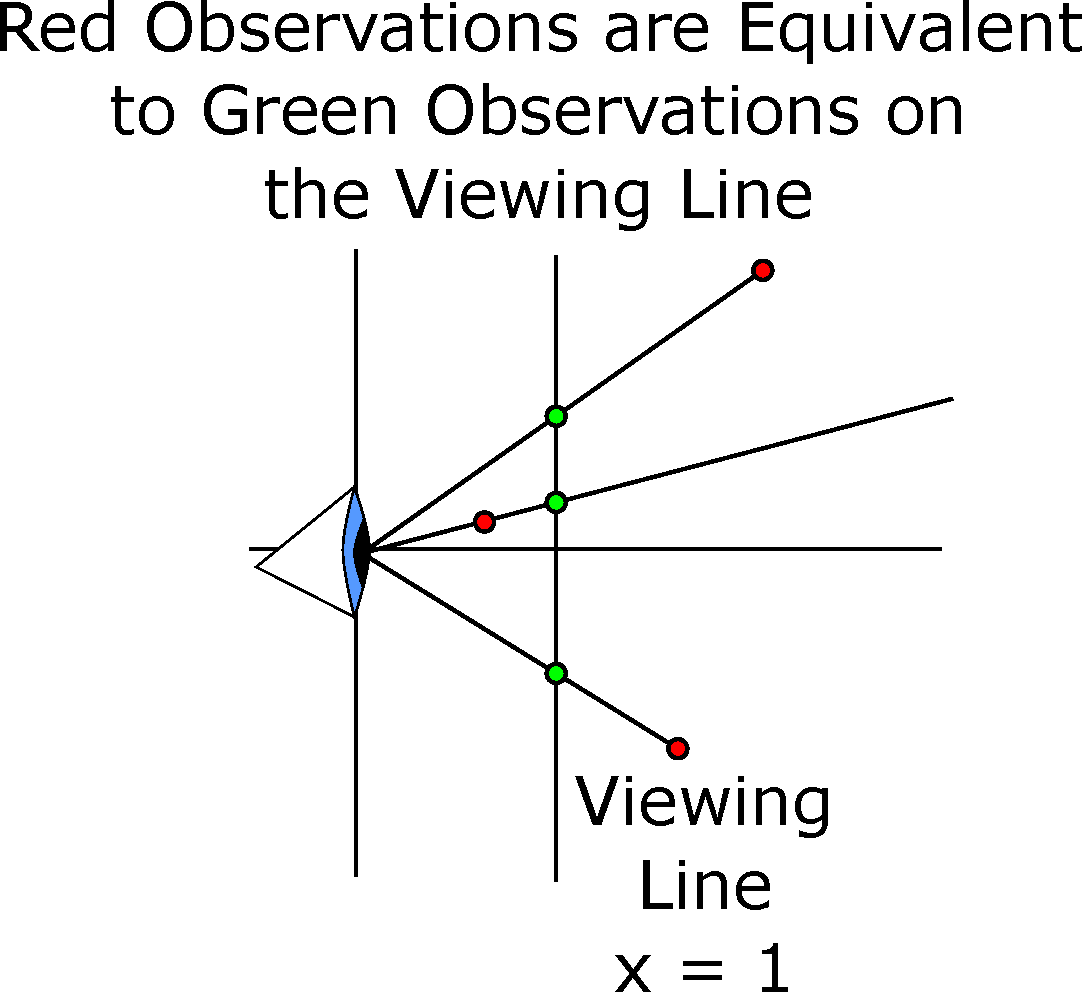
\includegraphics[width = 2in]{oneVarDiffCalc/perspective1.pdf}
\end{figure}

Now imagine that the eye rotates \(\pi/4\) radians counter-clockwise; it is now looking down a line that makes
an angle of \(\pi/4\) radians with the x-axis. Furthermore, its viewing line has rotated to be the 
line \(\left\{y + x = 2\sqrt{\frac{1}{2}} \right\}\). Let \(\tilde y\) denote the position along this 
new viewing line. See the figure below

\begin{figure}[h]
\centering
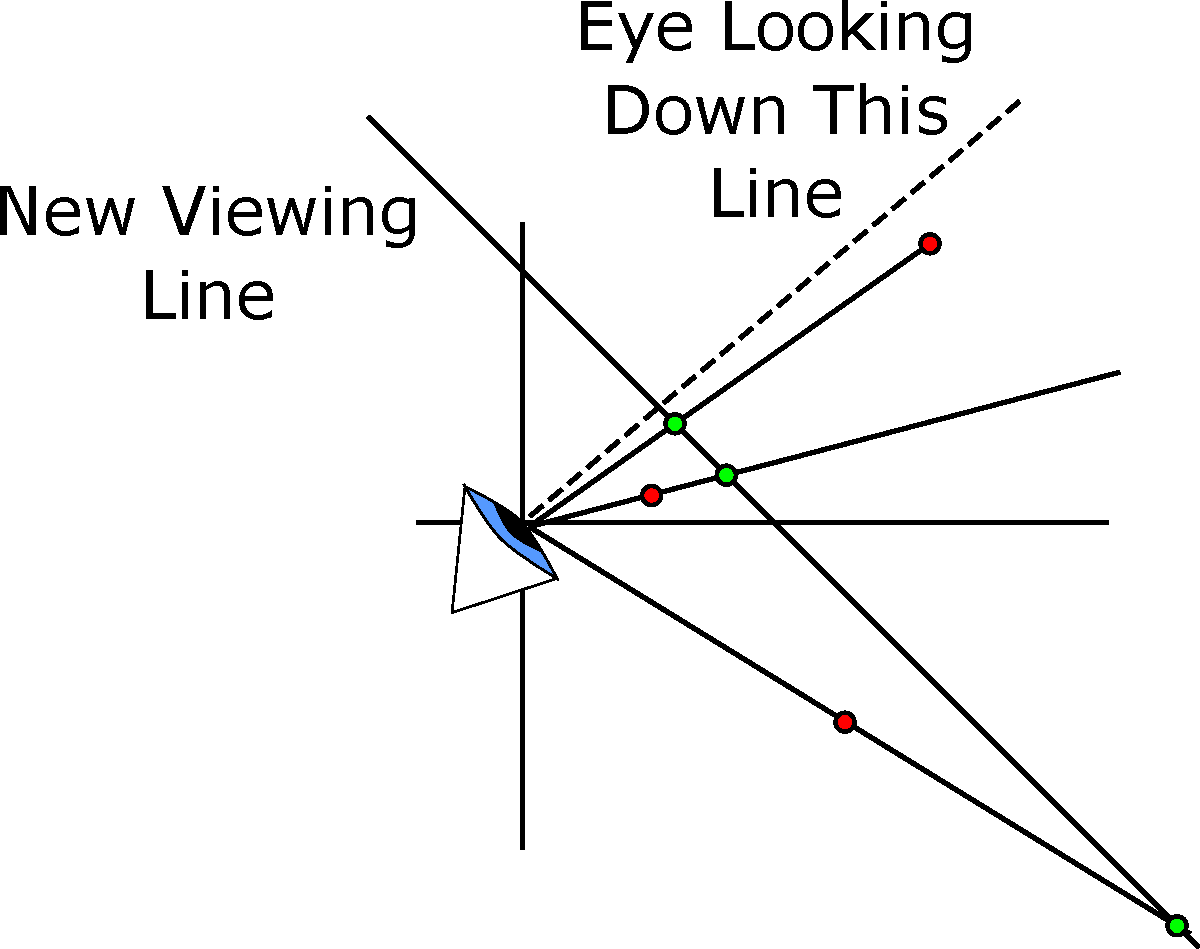
\includegraphics[width = 2in]{oneVarDiffCalc/perspective2.pdf}
\end{figure}

Let \(\tilde y\) measure position on the viewing line relative the line \(\{y = x\}\), i.e. the line that eye is
looking down. If an object appears to be at a point \(y\) on the original viewing line, what is its new position \(\tilde y\) on 
the new viewing line?
The answer turns out to be a linear fractional transformation, i.e.
\begin{equation}
\tilde y = \frac{A + By}{C + Dy},
\end{equation} 
for some constants \(A, B, C,\) and \(D\) depending on the angle of rotation.

Linear fractional transformations are also a classical topic in complex analysis, projective geometry, and
conformal geometry.

\subsubsection*{Finding the Schwarzian Derivative}

Now we will discuss our method of finding the Schwarzian derivative \(Su\) of a function \(u: \mathbb R \to 
\mathbb R\). We will demand that \(Su\) has the following properties:

\begin{enumerate}
\item The Schwarzian derivative is defined by
\begin{equation}
Su = F(u, u', u'', u'''),
\end{equation}
for some function \(F(a, b, c, d)\).

\item Given any function \(u(x)\) and linear fractional transformation \(T(y) = \frac{A + By}{C + Dy}\), we have
that the function defined by
\begin{equation}
w(x) = T(u(x)) = \frac{A + Bu(x)} {C + Du(x)},
\end{equation}
satisfies \(Sw = Su\).
\end{enumerate}

You can interpret the Schwarz derivative via perpective transformations. Suppose there is a particle moving in a
2-dimensional plane and the eye from our first set-up in the previous section observes it at position \(u(t)\)
in its viewing line. Next, suppose another observer is at 45 degrees relative to the first observer (so the 
second set-up) and observes the particle at position \(w(t)\) on their viewing line. Furthermore, suppose
neither observer knows the distance of their viewing plane and doesn't know the angle difference of
their perspectives. Is there some measure of the rate of change in the particle's position that they can agree on?

Yes, the Schwarzian derivative. Their observations differ by some linear fractional transformation; 
since they are missing data on their perspectives, they can't reconstruct the actual position of the particle
and they also can not reconstruct the details of the linear fractional transformation that relates their observations.
However, the Schwarzian derivative will always be the same despite no knowing the exact transformation. It is
enough to just know that it is a linear fractional transformation. 

\subsubsection*{The Problem}

Given the two properties of the Schwarzian derivative listed above, show that
\begin{equation}
F(u, u', u'', u''') = J\left( \frac{u'''}{u'} - \frac{3}{2} \left(\frac{u''}{u'}\right)^2 \right),
\end{equation}
for some function \(J\). Thus, deduce that a reasonable definition of the Schwarzian derivative is
\begin{equation}
Su = \frac{u'''}{u'} - \frac{3}{2}\left( \frac{u''}{u'} \right)^2.
\end{equation} 

\subsubsection*{The Solution}

First, we start by looking at the consequences of having an invariant for translations \(T(y) = A + y\) which
are fractional transformations for \(B = 1, C = 1,\) and \(D = 0\). Note that the derivatives of \(u\) and \(w\)
are equal. So we get that for any function \(u\) that
\begin{equation}
F(u + A, u', u'', u''') = F(u, u', u'', u''').
\end{equation}
Now, note that for any point \((a, b, c, d)\), we can find a function \(u\) such that 
\((u, u', u'', u''') = (a,b,c,d)\) for some point \(x\). So we get that
\begin{equation}
F(a + A, b, c, d) = F(a, b, c, d),
\end{equation} 
for any \(A, a, b, c,\) and \(d\). In particular, since we can vary \(A\) without changing the right
hand side, we see that the value \(F(a, b, c, d)\) is actually independent of \(a\). Therefore, we
may find a function \(G(b, c, d)\) such that
\begin{equation}
F(a, b, c, d) = G(b, c, d).
\end{equation}
Note that \(G(u', u'', u''')\) will be invariant for linear fractional transformations of \(u\) and 
that \(G(u', u'', u''')\) depends only on the derivatives of \(u\).

Next, we consider the effect of scalings \(T(y) = By\), these are also a specific class of linear fractional
transformations. We have that
\begin{equation}
G(Bu', Bu'', Bu''') = G(u', u'', u'''),
\end{equation}
for any \(B\). Similar to before, we get that
\begin{equation}
G(Bb, Bc, Bd) = G(b, c, d),
\end{equation}
for any \(B, b, c,\) and \(d\). Therefore, we see that \(G\) must be homogeneous of degree 0, i.e.
\begin{equation}
G(\lambda b, \lambda c, \lambda d) = G(b, c, d),
\end{equation}
for any constant scaling \(\lambda\).

Next, we consider the specific linear fractional transformation \(T(y) = \frac{1}{y}\). We then have that
\begin{align}
w & = \frac{1}{u}, \\
w' & = -\frac{u'}{u^2}, \\
w'' & = \frac{2u'^2}{u^3} - \frac{u''}{u^2}, \\
w''' & = \frac{6u'u''}{u^3} - \frac{6u'^3}{u^4} - \frac{u'''}{u^2}. 
\end{align}
So from the invariance of \(G\), we get that
\begin{equation}
G(u', u'', u''') = G\left( -\frac{u'}{u^2},
    \frac{2u'^2}{u^3} - \frac{u''}{u^2},
    \frac{6u'u''}{u^3} - \frac{6u'^3}{u^4} - \frac{u'''}{u^2} \right). 
\end{equation}
Now use the 0-homoegeneity of \(G\) to get
\begin{equation}
G(u', u'', u''') = G\left(-1, 
    \frac{2u'}{u} - \frac{u''}{u'}, 
    \frac{6u''}{u} - \frac{6u'^2}{u^2} - \frac{u'''}{u'}\right)
\end{equation}
Note that the expression on the right hand side contains terms involving \(u\) without any derivatives,
which isn't directly supplied as an argument to \(G\) on the left hand side. So when like before we
pass to general coordinates, the \(u\) terms turn into general constants \(A\). So we get
\begin{equation}
G(b, c, d) = G\left(-1, 
    \frac{2b}{A} - \frac{c}{b}, 
    \frac{6c}{A} - \frac{6b^2}{A^2} - \frac{d}{b}\right),
\end{equation} 
for any constant \(A\). So there exists a function \(H\) such that
\begin{equation}
G(b, c, d) = H\left(
    \frac{2b}{A} - \frac{c}{b}, 
    \frac{6c}{A} - \frac{6b^2}{A^2} - \frac{d}{b}\right),
\end{equation}
for any constant \(A\).

The fact that \(A\) is any general constant that appears on the right hand side but is not on the left means that 
there is more information to draw from \(H\). Let \(\theta = \frac{2b}{A} - \frac{c}{b}\). So
\begin{align}
\frac{6c}{A} - \frac{6b^2}{A^2} - \frac{d}{b} & = 
    \frac{3c}{b}\left(\theta + \frac{c}{b}\right)
    - \frac{3}{2}\left(\theta + \frac{c}{b}\right)^2 - \frac{d}{b}, \\
& = 3\left(\theta + \frac{c}{b}\right)\left(\frac{c}{2b} - \frac{\theta}{2}\right) - \frac{d}{b}, \\
& = \frac{3}{2}\left(\frac{c^2}{b^2} - \theta^2\right) - \frac{d}{b}.
\end{align}

So, we get that
\begin{equation}
G(b,c, d) = H\left(\theta, \frac{3}{2}\left(\frac{c^2}{b^2} - \theta^2\right) - \frac{d}{b} \right).
\end{equation}
Now, freeze \(b, c\) and \(d\) while varying \(A\). The left hand side is constant, but the value of \(\theta\)
on the right hand side is varying. So we see that the right hand side is constant on \(\{\theta < -\frac{c}{b}\}\) 
and it is also constant on \(\{\theta > -\frac{c}{b}\}\). Note as long as \(c \neq 0\) and \(b \neq 0\), we can
find a value of \(A\) such that \(\theta = 0\). So we have
\begin{equation}
G(b, c, d) = H\left(0, \frac{3}{2}\left(\frac{c}{b}\right)^2 - \frac{d}{b}\right),
\end{equation}
as long as \(c \neq 0\) and \(b \neq 0\).

So for \(b, c\neq 0\), we can write
\begin{equation}
G(b,c, d) = J\left(\frac{d}{b} - \frac{3}{2}\left(\frac{c}{b}\right)^2 \right).
\end{equation} 
As long as \(J\) is continuous, it extends to \(b \neq0\). So putting it all together, we get
\begin{equation}
F(u, u', u'', u''') = J\left( \frac{u'''}{u'} - \frac{3}{2}\left(\frac{u''}{u'}\right)^2 \right).
\end{equation}
We may take the expression inside parenthesese on the right hand side to be the Schwarzian derivative, i.e.
\begin{equation}
Su = \frac{u'''}{u'} - \frac{3}{2} \left(\frac{u''}{u'}\right)^2.
\end{equation}
You can now directly verify that if \(w(x) = T(u(x))\) for a linear fractional transformation \(T\), then
\(Sw = Su\).

\section{One Variable Integral Calculus}

\subsection{The Mercator Map and the Integral of Secant}

\subsubsection*{Historical Motivation}

The Mercator Map of the world spaces out the lines of latitude in a particular way inorder to solve a problem in naval navigation. 
The problem is that ships would navigate by sailing with a fixed angle to due north (e.g. as seen on a compass). 
This creates an issue for making map. 
Consider a map where the lines of latitude are spaced out evenly in the vertical direction (so NOT the Mercator map); for such a map, a course with fixed angle to magnetic north is NOT a straight line on the map.  

The problem is that the lines of latitude get represent shorter and shorter distances as you move from the equator towards either of the poles. 
This means that there is a complicated relationship between the angle measured on this map and the true angle to magnetic north it represents.

In 1569, Mercator had the idea that he could create a map where the lines of latitude are NOT spaced evenly; if you choose the variation in spacing in the correct manner, then a course with fixed angle to magnetic north will be a straight line on this new map. 
Furthermore, the angle measured on the map will match the true angle to magnetic north.

Unfortunately, Mercator didn't give a clear formula to precisely describe how to space out the lines of latitude. 
However, in 1599, Edward Wright found a precise mathematical description of how to space out the lines; he found that the spacing depended on the area under the secant function.
He didn't know how to precisely compute this area, but he was able to approximate it. 

Later in the 1640's, Henry Bond looked at a table of these approximate areas and a table of logarithms of trigonometic functions. 
He noticed a similarity in the two tables, and he was able to conjecture a precise formula for the area under the secant function. 
We now know that his conjecture was correct, but at the time there was no proof beyond numerical tables.

A proof was later given by Isaac Barrow; this proof is the earliest known publication of the use of integration by partial fractions.

\subsubsection*{The Problem}

Compute the integral
\begin{equation}
\int\limits_0^x \sec(u) \du.
\end{equation}

\subsubsection*{The Solution}

Recall that \(\sec(u) = \frac{1}{\cos(u)}\). First, let's use algebraic manipulation combined with the trigonometric formula \(\cos^2(u) + \sin^2(u) = 1\).
\begin{align}
\int\limits_0^x \frac{1}{\cos(u)} \du & = \int\limits_0^x \frac{\cos(u)}{\cos^2(u)} \du, \\
    & = \int\limits_0^x \frac{\cos(u)}{1 - \sin^2(u)} \du.
\end{align}

Now, we do a \(u\)-substitution. However, we are already use the variable \(u\), so let's make it a "\(w\)-substitution". 
We use \(w = \sin(u)\), and so \(\dw = \cos(u) \du\). Then we have that our integral is:
\begin{equation}
\int\limits_0^{\sin(x)} \frac{1}{1 - w^2} \dw.
\end{equation}
 Now, we use partial fractions: 
\begin{align}
\frac{1}{1 - w^2} & = \frac{1}{(1 - w)(1 + w)},\\
    & = \frac{A}{1 - w} + \frac{B}{1 + w}.
\end{align}

Combining terms and comparing numerators, we get \(A + B + (A - B)w = 1\). So we have
\begin{equation}
\begin{cases}
A + B = 1, \\
A - B = 0.
\end{cases}
\end{equation}
Solving we get \(A = B = \frac{1}{2}\).

Therefore, our integral becomes
\begin{align}
\int\limits_0^{\sin(x)} \frac{1}{2(1 - w)} + \frac{1}{2(1 + w)} \dw 
    & = \left. \frac{1}{2} \log\left(\frac{1 + w}{1 - w}\right)\right|_0^{\sin(x)}, \\
    & = \frac{1}{2} \log\left(\frac{1 + \sin(x)}{1 - \sin(x)}\right).
\end{align}

To simplify things, we can now use some trigonometric identities.
\begin{align}
\frac{1}{2} \log\left(\frac{1 + \sin(x)}{1 - \sin(x)}\right) & = \log\sqrt{\frac{1 + \sin(x)}{1 - \sin(x)}}, \\
    & = \log\sqrt{\frac{(1 + \sin(x))^2}{1 - \sin^2(x)}}, \\
    & = \log\left(\frac{1 + \sin(x)}{\cos(x)}\right), \\
    & = \log(\sec(x) + \tan(x)).
\end{align}

\subsection{Quadrature of the Hyperbola and Logarithms}

Now we investigate the relationship between the area under the graph of the hyperbola \(y = 1 / x\) and 
logarithms.

\subsubsection*{The Setup}

John Napier created the logarithm with the purpose of aiding in computations of multiplication and division. \cite{cajori} 
He noted that comparing an arithmetic progression to a geometric progression would allow one to, e.g., switch from
division to subtraction. By having a logarithm table, one can make division easier by converting to the
logarithm using the table, performing subtraction, and then using the logarithm table to convert back. 

So the original intention of logarithms is to take advantage of the algebraic fact that 
\begin{equation}
\log(ab) = \log(a) + \log(b).
\end{equation}

The relationship between logarithms and the area under the hyperbola \(y = 1/x\) was established by the work
of Gregory St. Vincent in 1647 and Alfons Anton de Sarasa in 1649 (note that their work is before the 
invention of calculus of Newton and Leibniz). Using modern terminology, we seek to show that 
\begin{equation}
f(x) \equiv \int\limits_1^x \frac{1}{t} dt,
\end{equation}
satisfies the algebraic rule of algorithms \(f(ab) = f(a) + f(b)\). Since this work predates the invention
of calculus, we will prove this result directly using methods of exhaustion, a technique that also predates
the invention of calculus.

\subsubsection*{The Problem}

\begin{enumerate}
\item Use a method of exhaustion to show that for any \(a, b, c > 0\), one has that
\begin{equation}
\int\limits_{ac}^{bc} \frac{1}{t} dt = \int\limits_a^b \frac{1}{t} dt.
\end{equation} 

\item Prove that
\begin{equation}
\int\limits_1^{ab} \frac{1}{t} dt = \int\limits_1^a \frac{1}{t} dt + \int\limits_1^b \frac{1}{t} dt.
\end{equation}
\end{enumerate}

\subsubsection*{The Solution}

\begin{enumerate}
\item First we partition \([ac, bc]\) using the points \(t_i = ac + \frac{bc - ac}{N} i \), for \(0 \leq i \leq N\).
Next, note that the points \(s_i = a + \frac{b - a}{N} i\) for \(0 \leq i \leq N\) give a partition of
the interval \([a, b]\).

Let \(U_N\) be the upper sum for the partition of \([ac, bc]\). We have that
\begin{align}
U_N & = \sum\limits_{i = 0}^{N-1} \frac{1}{t_i} \frac{bc - ac}{N}, \\
    & = \sum\limits_{i = 0}^{N - 1} \frac{1}{a + \frac{b - a}{N}i} \frac{b - a}{N}, \\
    & = \sum\limits_{i = 0}^{N - 1} \frac{1}{s_i} \frac{b - a}{N}, \\
\end{align}
Let us relate this to \(\int_a^b 1/t dt\). Now, we see that \(U_N\) isn't quite a lower bound for this integral.
However, we do have that it gives a lower bound for a slightly different interval. Let 
\(\delta_N = \frac{b - a}{N}\), we have that
\begin{equation}
U_N < \int\limits_{a - \delta_N}^{b - \delta_N} \frac{1}{t} dt.
\end{equation}

Similarly let the lower sum be \(L_N\); we have that 
\begin{align}
L_N & = \sum\limits_{i = 0}^{N-1} \frac{1}{t_{i+1}} \frac{bc - ac}{N}, \\ 
    & = \sum\limits_{i = 0}^{N - 1} \frac{1}{a + \frac{b - a}{N}(i+1)} \frac{b - a}{N}, \\
    & = \sum\limits_{i = 0}^{N - 1} \frac{1}{s_{i + 1}} \frac{b - a}{N}, 
\end{align}
We also see that
\begin{equation}
L_N > \int\limits_{a + \delta_N}^{b + \delta_N} \frac{1}{t} dt.
\end{equation}

So we have that
\begin{equation}
\int\limits_{a + \delta_N}^{b + \delta_N} \frac{1}{t} dt < \int\limits_{ac}^{bc} \frac{1}{t} dt
<  \int\limits_{a - \delta_N}^{b - \delta_N} \frac{1}{t} dt.
\end{equation}

As we let \(N \to \infty\), we have that \(\delta_N \to 0\). Therefore, we get that
\begin{equation}
\int\limits_a^b \frac{1}{t} dt \leq \int\limits_{ac}^{bc} \frac{1}{t} dt
    \leq \int\limits_a^b \frac{1}{t} dt.
\end{equation}
Therefore,
\begin{equation}
\int\limits_{ac}^{bc} \frac{1}{t} dt = \int\limits_a^b \frac{1}{t} dt.
\end{equation}

\item Next, consider the area
\begin{equation}
\int\limits_1^{ab} \frac{1}{t} dt.
\end{equation} 
From our previous result, we have that
\begin{equation}
\int\limits_{a}^{ab} \frac{1}{t} dt = \int\limits_{1}{b} \frac{1}{t} dt.
\end{equation}

Next, note that 
\begin{equation}
\int\limits_a^{ab} \frac{1}{t} dt = \int\limits_1^{ab} \frac{1}{t} dt - \int\limits_1^a \frac{1}{t} dt.
\end{equation}
Therefore, we get that
\begin{equation}
\int\limits_1^{ab} \frac{1}{t} dt = \int\limits_1^a \frac{1}{t} dt + \int\limits_1^b \frac{1}{t} dt.
\end{equation}

\end{enumerate}

\subsection{Volume of Particular Tori by Exhaustion}

In this section we look at using a method of exhaustion/rearrangement to evaluate a torus created from rotating
a 2-dimensional cross-section that has a vertical line of symmetry. 

\subsubsection*{The Setup}

The volume of a solid of revolution is provided by the classic Pappus' Centroid Theorem. The
theorem is mainly attributed to Pappus of Alexandria and Paul Guldin. Now, Pappus is a
mathematician of ancient Greece, and Guldin wrote his manuscript containing the theorem,
\textit{De centro gravitatis trium specierum quanitatis continuae} in 1640 (two years before
Newton was born). Typically this theorem is presented using integral calculus. However, given
that the creators of the theorem predate the invention of integral calculus, we are lead to wonder
if we can prove the theorem more directly using a method of exhaustion.

Here we will prove the theorem in the case that the cross-section of the revolution has a vertical
line of symmetry, much like in the figure below.

\begin{figure}[h]
\centering
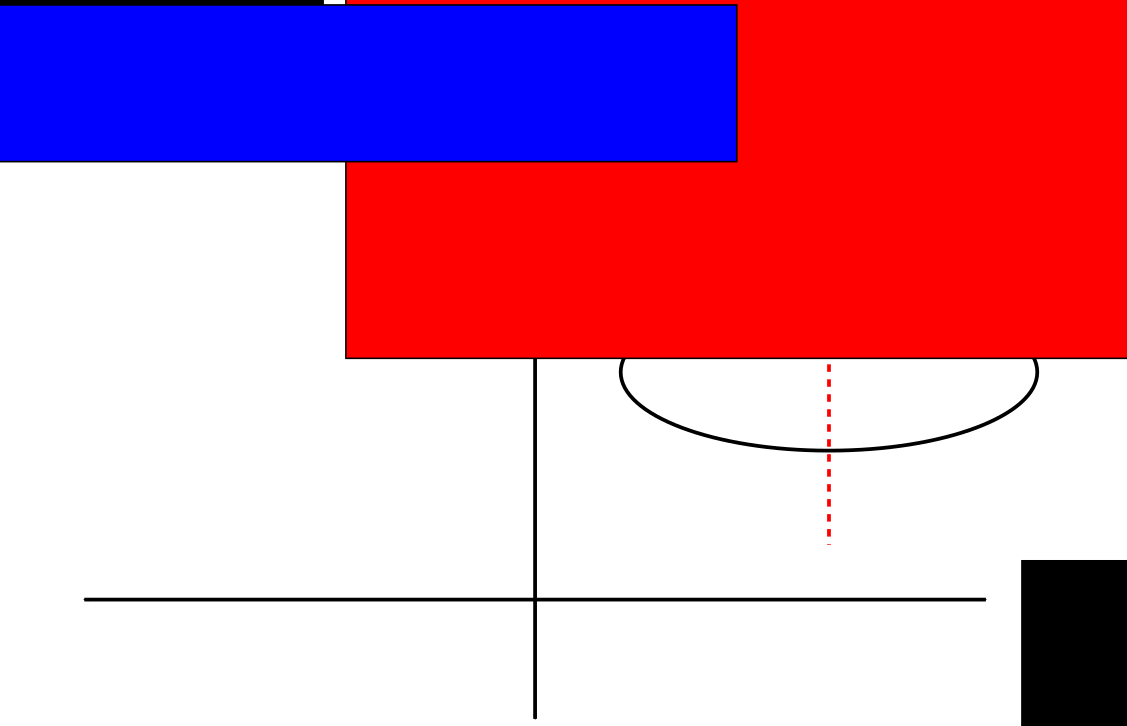
\includegraphics[width = 0.7 \textwidth]{_generated/pappus_cross_section.pdf}
\end{figure}

\subsubsection*{The Problem}

Given that the cross-section of the body of revolution has a vertical line of symmetry, find a
method of exhaustion/rearrangement that will compute its volume.

\subsubsection*{The Solution}

We divide the body of revolution into \(4n\) pieces by the angle of revolution, i.e. a number of 
pieces that is a multiple of four. For example, in the figure below is a picture of such a partition
from above.
\begin{figure}[h]
\centering
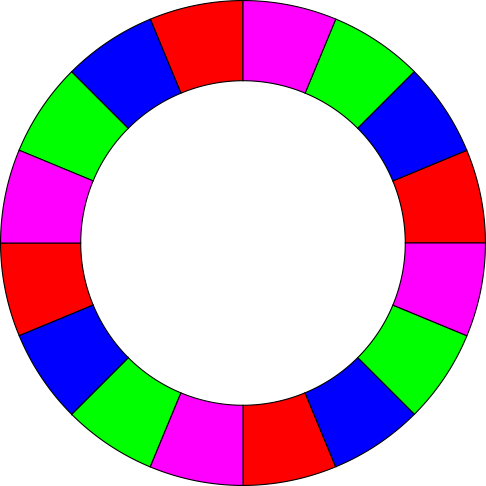
\includegraphics[width = 0.5 \textwidth]{_generated/pappus_exhaustion01.pdf}
\end{figure}

Since the cross-section has a vertical line of symmetry, if we take any piece and flip it to
rotate in the opposite direction, the ends of that piece can still be made to line-up with the
previous piece. Doing so, we can rearrange the pieces to "snake" back and forth. We use a number
of pieces that are a multiple of four, because this way the endpoints of the "snake" will be
aligned. See the figure below,

\begin{figure}[h]
\centering
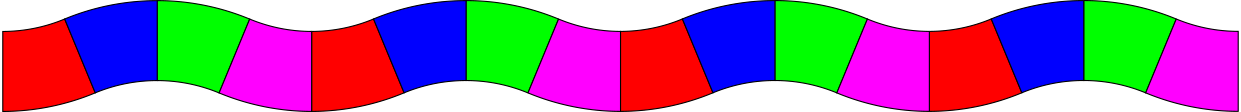
\includegraphics[width = 0.5 \textwidth]{_generated/pappus_exhaustion02.pdf}
\end{figure} 

Now, intuitively, as we make the number of pieces larger, the "snake" gets closer to a straight
cylinder. We see that each side of the cylinder is made of an equal number of pieces of arcs
coming from the "outer" circle of revolution as the "inner" circle of revolution. Let these
radii be \(r_1\) and \(r_2\). Then, intuitively we should have that sides of the cylinder are
\(2\pi(r_1 + r_2)/2\).

Let us prove this more rigorously.

Now, for each arc coming from the outer radius \(r_2\), from elementary geometry we have that the
width of the arc (NOT the length) is exactly
\begin{equation}
w_{\text{piece}} = 2r_2\sin\left(\frac{\pi}{4n}\right).
\end{equation}
Similarly for \(r_1\).

So we get that the total width of the snake is
\begin{equation}
w_n = 4n r_1 \sin\left(\frac{\pi}{4n}\right) + 4n r_2 \sin\left(\frac{\pi}{4n}\right).
\end{equation}
So \(w_n \to \pi r_1 + \pi r_2\). This is equal to the circumference of the circle formed by the
centroid of the cross-section (the symmetry of the cross-section gives us that the centroid has
radius \((r_1 + r_2)/2\)).

Technically, this last limit used that \(\frac{\sin(\theta)}{\theta} \to 1\) as \(\theta \to 0\).
This doesn't need to the full force of calculus to be shown as it follows from the classical
argument of comparing areas of triangles to areas of circular regions.

Now, we need lower and upper bounds on the volume of each rearrangement depending on \(n\). Look
at four consecutive segments of the "snake" and project their faces onto the plane of the base of
the "snake". We can use the areas of the intersections and the unions of these projections to give
us lower and upper bounds on the volume of the "snake" (which is equal to the volume of the
revolution). This is due to the face that snake is between the cylinder formed by the intersection
of the proejections and the cylinder formed by the union of the projections.

See the figures below for the pictures of the intersections and unions of the projections.
\begin{figure}[h]
\centering
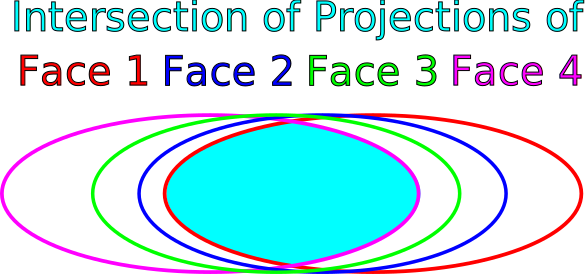
\includegraphics[width = 0.7 \textwidth]{_generated/pappus_intersection.pdf}
\end{figure}

\begin{figure}[h]
\centering
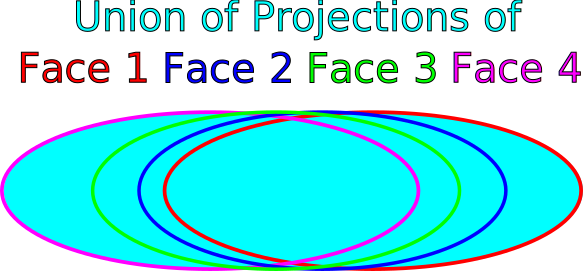
\includegraphics[width = 0.7 \textwidth]{_generated/pappus_union.pdf}
\end{figure}

Let the area of the intersection be \(I_n\) and the area of the union by \(U_n\). So we see that
the volume \(V\) of the body of revolution is bounded by
\begin{equation}
I_n w_n \leq V \leq U_n w_n.
\end{equation}

How it should be clear that are the number of pieces gets larger, the areas \(I_n\) and \(U_n\) get
closer to the area of the original cross section \(A\). Furthermore, we already showed that
\(w_n \to 2\pi r_{\text{centroid}}\). So from the pinching theorem, we get that
\begin{equation}
V = 2\pi r_{\text{centroid}} A.
\end{equation} 

\subsection{Fermat's Quadrature of the Folium of Descartes}

\subsubsection*{The Setup}

In this section we investigate how Fermat was able to use integration by parts to find the area of the
loop in the Folium of Descartes. A reference for Fermat's treatment of this problem is given by \cite{fermatTreatise}. 

The Folium of Descartes is the curve given by
\begin{equation}
x^3 + y^3 = 3C xy,
\end{equation}
where \(C\) is a constant. A graph of the curve for \(C = 1\) is given below. The curve crosses itself
at the origin.

\begin{figure}[h]
\centering
\includegraphics[width=3in]{oneVarIntCalc/graphFoliumDescartes.pdf}
\end{figure}

Fermat's idea comes in two parts:
\begin{enumerate}
\item If we can make a substitution for a new variable \(z\) to replace \(y\) given by \(y = C^{1 - m - n} x^m z^n\) such that the equation
now becomes
\begin{equation}
x^p = \sum\limits_{i} D_i^{p - p_i} z^{p_i},
\end{equation}
then we know how to compute the integral
\begin{equation}
\int\limits x^p dz.
\end{equation}
A note here about the choice of \(C^{1 - m - n}\), Fermat likes to follow the rules of homogeneity, which is probably best explained
in terms of units. If \(x\) and \(y\) were distances in say meters, then the left hand side of \(x^3 + y^3 = 3Cxy\) has units 
\(\text{meters}^3\). Fermat chooses a constant \(C\) that is also in meters, and so the right hand side also has units
\(\text{meters}^3\). Similarly, the left and right hand sides of \(y = C^{1 - m -n} x^m z^n\) have units of just meters. 

\item Use integration by parts to write the original area integral in terms of the integral we now know how to compute. That is, 
we try to find \(p\) and \(p_i\) to ensure that
\begin{equation}
\int\limits_0^{\bar x} (y_2 - y_1) dx = \int\limits_0^{\bar z} x^p dz.
\end{equation}  
It may be that \(\bar z = \pm \infty\), and so to be rigorous we will need to take an improper integral.
\end{enumerate}

\subsubsection*{The Problem}

Do the two steps of Fermat's plan to evaluate the area of the loop in the Folium of Descartes.

\subsubsection*{The Solution}

\begin{enumerate}
\item Let's do step one; let's make the substitution \(y = C^{1 - m - n} x^m z^n\) into \(x^3 + y^3 = 3Cxy\). We get
\begin{equation}
x^3 + C^{3 - 3m - 3n} x^{3m} z^{3n} = 3C^{2 - m - n} x^{1 + m} z^n.
\end{equation}
Let's us now try to consolidate the \(x\)-terms into one term \(x^p\); to do so, two of the terms need to have the same power of \(x\). 
Let's look at the three cases:
    \begin{enumerate}
    \item If we try equating \(x^3 = x^{3m}\), then we must have \(m = 1\). So we get
    \begin{equation}
    1 + C^{-3n} z^{3n} = 3C^{1 - n} x^{-1} z^n.
    \end{equation} 
    Consolidating the z-terms, this becomes
    \begin{equation}
    3C^{1 - n} x^{-1} = z^{-n} + C^{-3n} z^{2n}.
    \end{equation}
    The problem here is that there is no way to produce the power \(x^{-1}\) using integration by parts without using a logarithm. So
    this case isn't really any help.

    \item Now let's try equating \(x^3m = x^{1 + m}\). We then have that \(m = \frac{1}{2}\). So we get
    \begin{equation}
    x^{3/2} = -C^{3/2 - 3n} z^{3n} + 3 C^{3/2 - n} z^n.
    \end{equation}   
    Again, we can't directly get \(x^{3/2}\) without introducing some radical power of \(x\) that isn't already present. We could just
    square the equation, but we will see that it is better to work with the last case.

    \item Now we equate \(x^3 = x^{1 + m}\) and we get \(m = 2\). So then we have that
    \begin{equation}
    1 + C^{-3 - 3n} x^3 z^{3n} = 3C^{-n} z^n,
    \end{equation}
    which gives us
    \begin{equation}
    x^3 = 3C^{3 + 2n} z^{-2n} -C^{3 + 3n} z^{-3n}. 
    \end{equation}
    The power \(x^3\) is a nice integer power for us to work with.
    \end{enumerate}

So we take \(y = C^{-1 - n} x^2 z^n\) where \(n\) is still left to be determined. Our equation defining the folium is now
\begin{equation}
x^3 = 3C^{3 + 2n} z^{-2n} - C^{3 + 3n} z^{-3n}.
\end{equation}

\item
Let us now consider the area integral
\begin{equation}
\int\limits_0^a (y_2 - y_1) dx = C^{-1 - n} \int\limits_0^a (z_2^n - z_1^n) x^2 dx
\end{equation}
When we perform integration by parts, we will get an integral of the form (ignoring the boundary terms for now)
\begin{equation}
\frac{n}{3}\int z^{n - 1} x^3 dz. 
\end{equation}
This is most simple when \(n = 1\). So we will take \(y = C^{-2} x^2 z\) for our variable transformation. The equation of the folium is now
\begin{equation}
x^3 = 3C^5 z^{-2} - C^6 z^{-3}.
\end{equation}
Now we need to be more rigorous with our boundary terms. 

First note that the loop of the folium of descartes is in the first quadrant, i.e. \(\{x,y \geq 0\}\). 
Furthermore, the only non-negative solutions to \(3C^5 z^{-2} - C^6 z^{-3} = 0 \) are \(z = \frac{C}{3}\) and \(z = \infty\). 

Next, note that for \(x^3 + y^3 = 3Cxy\) and \(x, y\) close to the origin, the \(3Cxy\) term dominates. So we expect the loop to
be asymptotically like \(3xy = 0\). That is, one direction of approach to the origin is horizontal while the other is vertical. We need
to investigate this asymptoticness more closely.

For any point \((x,y)\) on the folium and close to the origin, let \(\lambda = \|(x,y)\|\) and let \((\tilde x, \tilde y) = \frac{1}{\lambda}(x, y)\). 
Using the equation for the folium, we have that 
\begin{equation}
0 \leq \tilde x \tilde y \leq \frac{\lambda}{3C}.  
\end{equation}
Note that \((\tilde x, \tilde y)\) occur on the unit circle. Consider the function \(f(x,y) = xy\) and its parameterization on the unit circle
given by \(g(\theta) = f(\cos\theta, \sin\theta) = \cos\theta \sin\theta\). Now note that where \(g\) vanishes for the first quadrant is \(\theta = 0\) or
\(\theta = \pi/2\). Furthermore, \(g'(0)\neq 0\) and \(g'(\pi/2) \neq 0\). 

We can use this and some basic trignometry to show that \(\tilde x \tilde y \leq \frac{\lambda}{3C}\) gives us that \(\|(\tilde x, \tilde y) - (1,0)\| \leq K \lambda\) or
\(\|(\tilde x, \tilde y) - (0, 1)\| \leq K \lambda\) for some constant \(K\) depending on \(C\).

The first case is the horizontal part of the loop approaching the origin. In this case, we have that \(z = C^2 y / x^2 = C^2 \frac{\tilde y} {\lambda \tilde x^2}\). Now, as we approach
the origin, \(\lambda \to 0\), \(\tilde x \to 1\) and \(\tilde y \leq K \lambda\). So we get that \(z\) is bounded as we approach the origin along the horizontal portion of the loop.
So it must approach \(z = \frac{C}{3}\).

The second case is the vertical portion of the loop approacing the origin. In this case, we write \(z = C^2 \frac{\tilde y}{x\tilde x}\). We have that \(\tilde x \to 0\), \(x \to 0\), and
\(\tilde y \to 1\). Therefore \(z \to \infty\) along the vertical portion of the loop as we approach the origin.

From the \(xz\)-equation of the folium, we see that in either case that \(zx^3 \to 0\) as \(x \to 0\). Now let us rigorously apply integration by parts.
We have that
\begin{align}
\int\limits_0^{\bar x} (z_2 - z_1) x^2 dx & = \lim\limits_{a \to 0+} \int\limits_a^{\bar x} (z_2 - z_1) d \left(\frac{x^3}{3}\right), \\
    & = \lim\limits_{a \to 0+} \frac{1}{3}(z_2 - z_1)x^3\big |_a^{\bar x} + \int\limits_{C / 3} ^ {\bar z}\frac{1}{3} x_1^3 dz + \lim\limits_{b \to\infty} \int\limits_{\bar z}^b x_2^3 dx, \\
    & = 0 + \lim\limits_{b\to\infty} \int\limits_{C/3}^b x^3 dz,\\
    & = \lim\limits_{b\to \infty} \int\limits_{C/3}^b 3C^5z^{-2} - C^6 z^{-3} dz, \\
    & = \lim\limits_{b\to \infty} \frac{C^6}{2}z^{-2} - 3C^5 z^{-1} \big|_{C/3}^b, \\ 
    & = 9C^4 - \frac{9}{2}C^4, \\
    & = \frac{9}{2}C^4.
\end{align} 

Combining with the area integral, we get
\begin{equation}
\int\limits_0^{\bar x} (y_2 - y_1) dx = \frac{9}{2}C^2.
\end{equation}
\end{enumerate}


\section{Multivariable Differential Calculus}

Here are examples related to differential calculus in more than one variable.

\subsection{Envelopes}

In the simplist cases, the \textbf{envelope} of a family \(\mathfrak F\) of curves is a curve \(\gamma\) that is in some sense extremal to the entire family of curves. 
What is often the case, is that every point of the curve \(\gamma\) touches exaclty one curve from the the family \(\mathfrak F\), and furthermore this touching is only tangential (i.e. they cross at an angle of zero). 
This is best illustrated with examples. 

\subsubsection{The Hyperbola as an Envelope}

\subsubsection*{The Set Up}

Consider the family \(\mathfrak F\) of straight lines in \(\mathbb R^2\), where each line crosses the x-axis and y-axis at pairs of points of the form \((s,0)\) and \((0, 1/s)\) for some \(s > 0\). 
So we see that each line is of the form \(\frac{1}{s} x + s y = 1\) for some \(s > 0\).
Some of the lines from the family are pictured in the following figure.

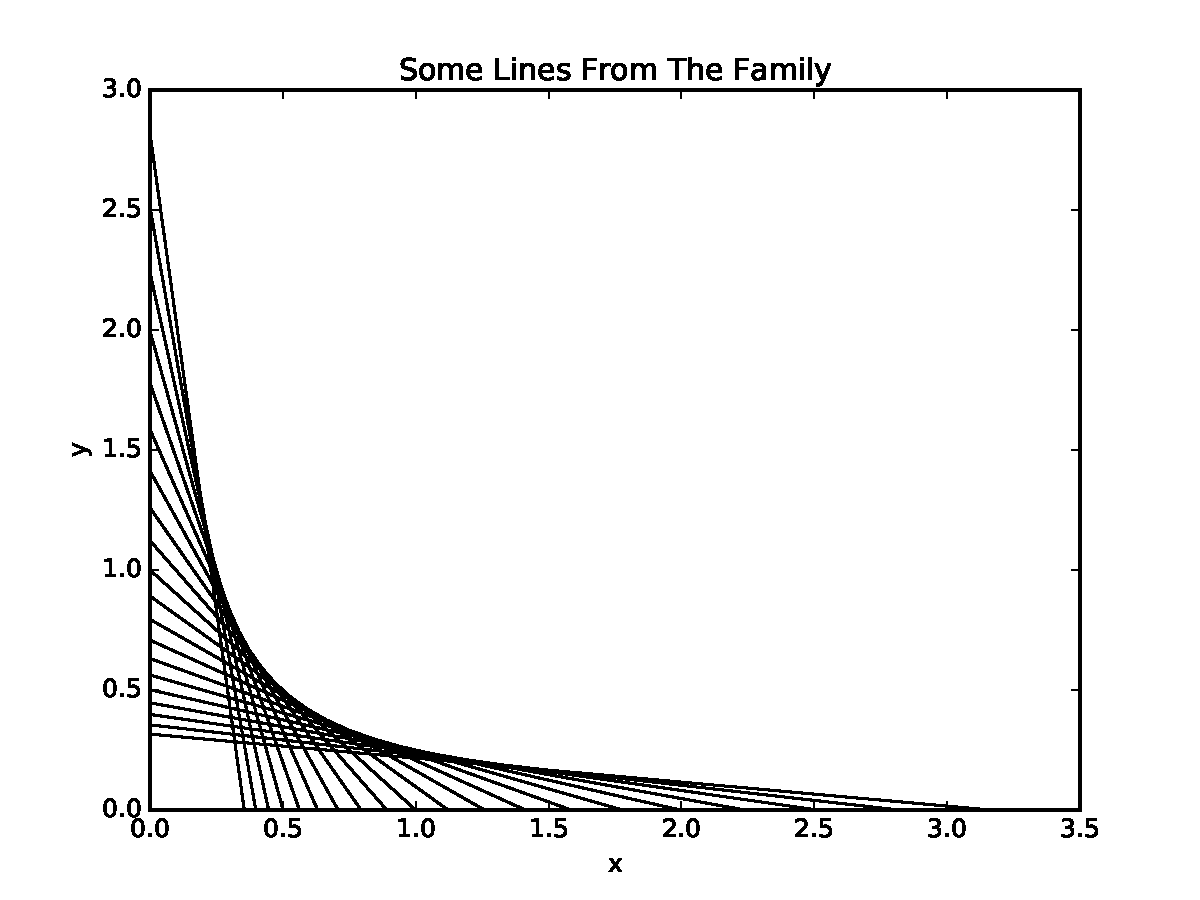
\includegraphics[width = 4.0in]{multiVarDiffCalc/hyperbolaFamily.pdf}

We can see that extemal to the family of lines is a curve concave up in the first quadrant \(\{x, y > 0\}\). In the following figure, you can see the curve superimposed with some of the lines from the family.

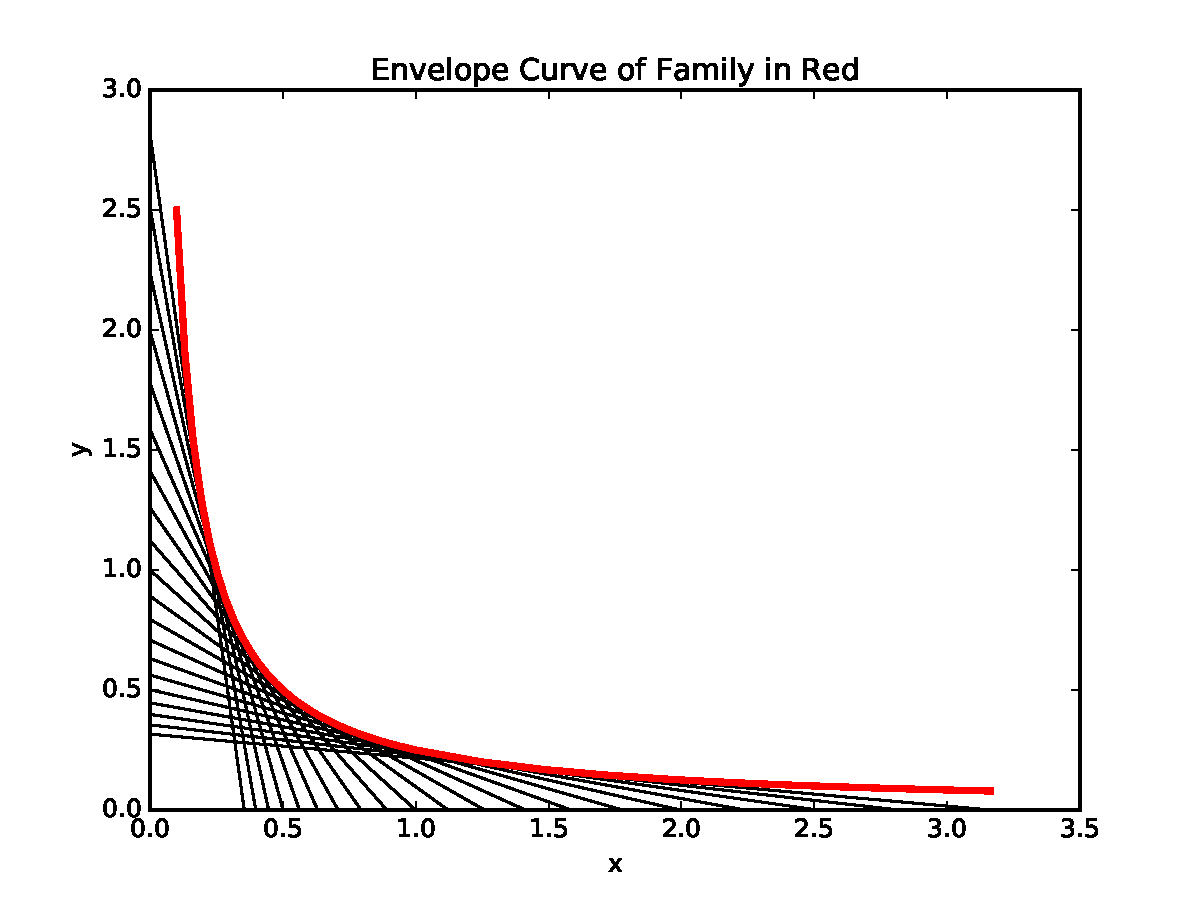
\includegraphics[width = 4.0in]{multiVarDiffCalc/hyperbolaEnvelope.pdf}

\subsubsection*{The Problem}
Let us consider computing the envelope curve \(\gamma(x)\) of the family \(\mathfrak F\). 

\subsubsection*{The Solution}

To compute the envelope curve \(\gamma(x)\), let us consider the auxilliary function
\(g(x,y,s) = \frac{1}{s} x + s y - 1\). Let us see how the Implicit Function Theorem of vector calculus let's us
use \(g(x,y, s)\) to find the exremal envelope curve \(\gamma(x)\). As we discuss this, please consider the similarities to the ordinary first derivative test.

First, consider any point \((x_0, y_0)\) NOT on the extremal envelope curve \(\gamma(x)\), but is touched by some line in \(\mathfrak F\). 
So there is some \(s_0 > 0\) such that \(\frac{1}{s_0} x_0 + s_0 y_0 = 1\); note that this is equivalent to \(g(x_0, y_0, s_0) = 0\). 
Since \((x_0, y_0)\) isn't on the boundary of the region of points touched by lines in \(\mathfrak F\), we know that for any other points \((x_1, y_1)\) close to \((x_0, y_0)\) we may find another line in \(\mathfrak F\) touching \((x_1, y_1)\). 
That is, for every \((x_1, y_1)\) close to \((x_0, y_0)\), we may find \(s_1 > 0\) such that \(g(x_1, y_1, s_1) = 0\).  

This can be summarized as saying that for all points \((x_0, y_0)\) that are touched by a line in \(\mathfrak F\) and also isn't on the envelope \(\gamma\), we can locally solve \(s = S(x,y)\) such that \(g(x, y, S(x, y)) = 0\). Now, you may begin to see the connection to the Implicit Function Theorem.

Recall that the Implicit Function Theorem can only confirm that we CAN locally solve \(s = S(x,y)\) such that \(g(x, y, S(x, y)) = 0\). However, we seek for the extremal points where we CAN'T locally solve. This is similar to the first derivative test of ordinary calculus. Technically, the first derivate test only says when a point is NOT an extemum of a function; then the candidate points for extrema are reduced to some finite list by solving for the vanishing of the derivative.

Here, we are in a similar situation. We solve for a set of candidate points that must contain our extremal curve \(\gamma\). 
It will happen to be the case that our candidate set will allow only one curve and so this must be the envelope.
However, we are being a little reckless here as we haven't proven the curve must exist; we will consider the picture to be very convincing and ignore this technical detail. 

So we seek for when we can't locally solve \(s = S(x,y)\) such that \(g(x, y, S(x, y)) = 0\). The Implicit Function Theorem tells us this will only be possible for those \((x,y,s)\) with \(g(x,y,s) = 0\) and \(\frac{\partial g}{\partial s} (x, y, s) = 0\).

So we look for
\begin{align}
0 & = \frac{\partial g}{\partial s}, \\
&  = -\frac{x}{s^2} + y
\end{align}

We wish to find an equation restricting \(x\) and \(y\); so it is most efficient to solve the above for \(s\). 
Also, from the picture it is clear that we should restrict to \(x, y > 0\). 
Therefore, for \(x, y > 0\), we have \(s = \sqrt{\frac{x}{y}}\). Plugging this into the equation for \(g(x, y, s) = 0\), we get 
\begin{equation}
\sqrt{xy} + \sqrt{xy} - 1 = 0.
\end{equation} 

Therefore, we find that the envelope curve must lie inside the set \(S = \{xy = \frac{1}{4}\}\). However, one will recognize that for each point \(x > 0\), there is only one \(y\) such that \(y \in S\). Therefore, the envelope must be this curve.

So the envelope \(\gamma(x)\) is the curve \(y = \frac{1}{4x}\) for \(x > 0\).  

\subsubsection*{Final Remark}

Note that the set \(S\) is actually a hyperbola. Therefore, the hyperbola can be realized as the envelope of a simple family of straight lines. For this reason, hyperbolas are (approximately) reproducible in "string art": art formed from
straight line segments where each segment is made by tightened string.

\subsection{Differentiable Function With Bounded Non-Continuous Derivatives}

\subsubsection*{Setup}

Functions that are differentiable everywhere do not necessarily have continuous derivatives, even if the derivatives of the function are bounded. For the case of one variable, a classic example is
\begin{equation}
f(x) = \begin{cases}
    x^2 \sin(\frac{1}{x}) & x\neq 0,\\
    0 & x = 0.
    \end{cases}
\end{equation}
Here, the altering of the amplitude by the factor of \(x^2\) forces the function to be differentiable at \(x = 0\) and \(f'(0) = 0\). This can be checked by directly applying the definition of differentiability. However, the derivative \(f'(x)\) alternates infinitely between values close to \(f' = -1\) and \(f' = 1\) as \(x \to 0\). Therefore, the function does not have continuous derivatives.

However, one may wonder if this "infinite frequency oscillation" is necessary. In this example, we show that this is unnecessary in two-dimensions. That is, we construct a function \(u(x,y)\) that is 
differentiable everywhere, has bounded derivatives, and does not have continuous derivatives at \((0,0)\).

\subsubsection*{The Problem}

Find a simple function \(u(x,y)\) such that \(u\) is differentiable on \(\mathbb R^2\), the derivatives of \(u\) are bounded, and at least one of the derivatives of \(u\) is NOT continuous at \((0,0)\).

\subsubsection*{The Solution}

First let us consider a phenomenon in one-variable calculus. If \(g(x)\) is a differentiable function with bounded derivatives: \(|g'| \leq M\), then for any constant \(\lambda > 0\) the function
\(h(x) = \lambda g\left(\frac{x}{\lambda}\right)\) has the same bound for its derivatives, i.e. \(|h'| \leq M\). This is easily proved using the chain rule:
\begin{align}
h'(x) & = \lambda \frac{d}{dx} \left( g\left(\frac{x}{\lambda}\right)\right), \\
    & = \lambda g'\left(\frac{x}{\lambda}\right) \frac{1}{\lambda}, \\
    & = g'\left(\frac{x}{\lambda}\right). 
\end{align}
Therefore, if \(|g'| \leq M\), then \(|h'| \leq M\) too. 

So the idea is that we can construct a function \(u(x,y)\) by setting \(u(x,y) = (x^2 + y^2) h\left(\frac{x}{x^2 + y^2}\right)\) for an appropriate function \(h(x)\). What properties should we require
of \(h(x)\)? First, let's check what is necessary for bounded derivates. Although we were guided by our idea in one-variable differentiation, we must now explicitly check that everything works out okay
since our factor \(x^2 + y^2\) isn't actually constant. 

First, let's calculate the \(x\)-derivative when \((x,y) \neq (0, 0)\):
\begin{align}
\frac{\partial u}{\partial x} & = 2x h + (x^2 + y^2) h' \left(\frac{1}{x^2 + y^2} - \frac{2x^2}{(x^2 + y^2)^2}\right), \\
    & = 2xh + h' - h' \frac{x^2}{x^2 + y^2}. 
\end{align}

Now, let's calculate the \(y\)-derivative when \((x,y) \neq (0,0)\):
\begin{align}
\frac{\partial u}{\partial y} & = 2yh + (x^2 + y^2) h' \frac{2xy}{(x^2 + y^2)^2}, \\
    & = 2yh + h'\frac{2xy}{x^2 + y^2}.
\end{align}

Therefore, we see that the derivatives \(u_x\) and \(u_y\) will be bounded for \((x,y) \neq (0,0)\) when the function \(h(x)\) and its derivative \(h'(x)\) are both bounded; note that expressions like
\(\frac{x^2}{x^2 + y^2}\) and \(\frac{2xy}{x^2 + y^2}\) are bounded for points away from the origin because they are invariant under scaling (i.e. homogeneous of order 0).

Finally, when \(h(x)\) is bounded, the fact that we mulitply \(h\) by \(x^2 + y^2\) to construct \(u\) implies that \(u\) will be differentiable at the origin and that \(u_x(0,0) = u_y(0,0) = 0\).
Now, focus on the expression \(h' \frac{2x^2}{x^2 + y^2}\) in the expression for \(u_x\). If we approach the origin along \(y^4 = x\), then
\begin{align}
h'\left(\frac{x}{x^2 + y^2}\right) & = h'\left(\frac{\sqrt{x}}{x^{3/2} + 1}\right) ,\\
    & \to h'(0).
\end{align} 
Furthermore as we approach the origin along \(y^4 = x\), 
\begin{align}
\frac{x^2}{x^2 + y^2} & = \frac{x^{3/2}}{x^{3/2} + 1}, \\
    & \to 0. 
\end{align}
Therefore, as we approach the origin along \(y^4 = x\), we have that \(u_x \to h'(0)\). So we will want \(h'(0) \neq 0\), e.g. \(h'(0) = 1\).

Let us recap our requirements for \(h(x)\).
\begin{itemize}
\item The function \(h(x)\) is differentiable with continuous derivatives on \(\mathbb R\)
\item The values of the function \(h(x)\) and its derivative \(h'(x)\) are both bounded.
\item At \(x = 0\), we have \(h'(0) = 1\).
\end{itemize}

A function that meets all of these requirements is \(h(x) = \frac{x}{1 + x^2}\). So our function \(u(x,y)\) is
\begin{align}
u(x,y) & = (x^2 + y^2) h\left(\frac{x}{x^2 + y^2}\right), \\
    & = (x^2 + y^2) \frac{x}{(x^2+y^2)(1 + x^2 (x^2 + y^2)^{-2})}, \\
    & = \frac{x(x^2 + y^2)^2}{(x^2 + y^2)^2 + x^2}.
\end{align}

\subsection{Maximizing Likelihood for a Three Step Markov Process}

\subsubsection*{The Setup : The Constraints}

\newcommand{\flip}[1]{\overline{#1}}

We have three random variables \(X_1\), \(X_2\), and \(X_3\) where each \(X_i = 0\) or \(X_i = 1\). The order
of the variables matter, and we think of them as randomly being chosen in sequence according to their indices
one, two, or three. 

So there are eight possible outcomes according to the two possible values for each \(X_i\); we label these
outcomes as \(X_1X_2X_3\), e.g. \(000\) or \(110\). We label the probabilities of the outcomes according to these  
possibilities, e.g. \(p_{000}\) or \(p_{110}\). We think of the probabilities forming a vector 
\(\vec p \in \mathbb R^8\), i.e. the vector \(\vec p = (p_{000}, p_{001}, ..., p_{111})\). 

Finally, one more notation we will use. We will use \(\flip i\) to denote the other value of \(0\) or \(1\) that 
is not \(i\); i.e. if \(i = 1\) then \(\flip i = 0\).

To be a three step Markov process, the transition from \(X_2\) to \(X_3\) needs to depend only on \(X_2\) and
not on the entire history, i.e. not depend on \(X_1\) and \(X_2\). In terms of probabilities, this is
expressed as 
\begin{equation}
P(X_3 = k | X_1 = i, X_2 = j) = P(X_3 = k | X_2 = j).
\end{equation}
Applying Bayes' formula to both sides of this equation, we get
\begin{equation}
\frac{p_{ijk}}{\sum_\gamma p_{ij\gamma}} 
= \frac{\sum_\alpha p_{\alpha jk}} {\sum_{\alpha, \gamma} p_{\alpha j\gamma} }.
\end{equation}
We can rewrite this as 
\begin{equation}
p_{ijk} \sum_{\alpha, \gamma} p_{\alpha j\gamma} =
     \left(\sum_\alpha p_{\alpha jk}\right) \left( \sum_\gamma p_{ij\gamma} \right).
\end{equation}
Next, let's expand the sums over \(\gamma\) as sums over the values \(k\) and \(\flip k\); we get
\begin{equation}
p_{ijk}\sum_\alpha p_{\alpha jk} + p_{ijk} \sum_\alpha p_{\alpha j\flip k} =
p_{ijk} \sum_\alpha p_{\alpha jk} + p_{ij\flip k} \sum_\alpha p_{\alpha jk}.
\end{equation}
Cancelling terms we get
\begin{equation}
p_{ijk} \sum_\alpha p_{\alpha j\flip k} = p_{ij\flip k} \sum_\alpha p_{\alpha jk}.
\end{equation}
Now expand the sum over \(\alpha\) as a sum over the values \(i\) and \(\flip i\), we get
\begin{equation}
p_{ijk} p_{ij\flip k} + p_{ijk} p_{\flip ij\flip k} = p_{ij\flip k} p_{ijk} + p_{ij\flip k} p_{\flip ijk}.
\end{equation}
Again, cancelling terms we get
\begin{equation}
p_{ijk} p_{\flip ij\flip k} = p_{ij\flip k} p_{\flip ijk}.
\end{equation}

Now, at first this appears to be eight different equations, one for each possible choice of \((i, j, k)\). 
However, we will now show that it is actually just two different equations without doing a brute force
plug and check.

First, notice that the equation is exactly the same if we make the substitution \(i \to \flip i\); the effect
is to merely switch the left and right hand side of the equation. Therefore, the equation is the same no matter
which value of \(i\) we choose. So let us choose \(i = 0\).

Similarly, using the substitution \(k \to \flip k\), we can choose \(k = 0\). Both of these choices give
\begin{equation}
p_{0j0} p_{1j1} = p_{0j1} p_{1j0},
\end{equation}
for either \(j = 0\) or \(j = 1\). It is not very hard to see that we get different equations for each
different value of \(j\). 

Therefore, we find that the constraints for \(\vec p\) to be a three step Markov process are exactly the
four following constraints: 
\begin{equation}
\begin{cases}
p_{ijk} \geq 0, \\
\sum_{\alpha, \beta, \gamma} p_{\alpha\beta\gamma} = 1, \\
p_{000} p_{101} = p_{001} p_{100}, \\ 
p_{010} p_{111} = p_{011} p_{110}.
\end{cases}
\end{equation}
All probability vectors \(\vec p \in \mathbb R^8\) that belong to three step Markov processes are exactly 
the probability vectors \(\vec p\in \mathbb R^8\) that satisfy all of the above constraints. 

\subsection*{The Setup: Maximizing Likelihood}

We are interested in creating statistical estimates for the different \(p_{ijk}\) based on data recording
sample counts \(n_{ijk}\); that is, we run \(N\) independent trials, and \(n_{ijk}\) is the 
number of times we see outcome \(X_1 = i\), \(X_2 = j\), and \(X_3 = k\). We denote the collection of
all the \(n_{ijk}\) as a vector \(\vec n\) similarly to how we used \(\vec p\) above. 

First, let us briefly discuss the notion of likelihood. For the notion of likelihood, you consider the
data \(\vec n\) to be fixed, and we consider varying the probabilities of our model \(\vec p\). The 
likelihood is defined as the probabilitiy \(l(\vec p) = P(\vec n | \vec p) \) for our three step Markov
model. Assuming the trials are independent, we have
\begin{equation}
l(\vec p) = \prod_{\alpha, \beta, \gamma} (p_{\alpha\beta\gamma})^{n_{\alpha\beta\gamma}}.
\end{equation} 
The term "likelihood" is used instead of probability, because \(l(\vec p)\) does not in general represent
a probability distribution on \(\vec p\).

The idea is that a good estimate of the true probabilities should come from finding \(\vec p\) that
maximizes the likelihood \(l(\vec p\). 

Next note that maximizing likelihood is equivalent to maiximizing the logarithm of likelihood; however,
the latter has a nicer form. So let \(L(\vec p) = \log(l(\vec p))\). We see that
\begin{equation}
L(\vec p) = \sum_{\alpha, \beta, \gamma} n_{\alpha\beta\gamma} \log(p_{\alpha\beta\gamma}).
\end{equation}

Now, recall that those \(\vec p\) that represent three step Markov processes are exactly those \(\vec p\) 
satisfying four constraints. So we are lead to a constrained maximization problem. We will assume that
the maximum occurs at the interior of the constraints, i.e. \(p_{ijk} > 0\) for all \((i, j, k)\). 

\subsubsection*{The Problem}

Let the data \(n_{ijk}\) be fixed. Assume that the maximum of the following constrained problem occurs at \(p_{ijk} > 0\) for all \((i, j, k)\):
\begin{equation}
\begin{cases}
\text{maximize } L(\vec p) = \sum_{\alpha, \beta, \gamma} n_{\alpha\beta\gamma} \log p_{\alpha\beta\gamma}, \\
\sum_{\alpha, \beta, \gamma} p_{\alpha\beta\gamma} = 1, \\
p_{0j0} p_{1j1} = p_{0j1} p_{1j0}, & \text{ for } j \in \{0, 1\}.
\end{cases}
\end{equation}

Find the \(p_{ijk}\) where the maximum occurs in terms of the data \(n_{ijk}\).


\section{Multivariable Integral Calculus}

\subsection{Function Not Satisfying Fubini's Theorem}

\subsubsection*{Set Up}

Here we consider Fubini's theorem in two-dimensions.

Fubini's theorem tells us two things:
\begin{itemize}
\item When we know we can compute a two-dimensional integral as a repeated application of one-dimensional integration over the variables \(x\) and \(y\).

\item When we know the order of the repeated one-dimensional integration over \(x\) and \(y\) doesn't depend on the order of integrating over \(x\) and \(y\). 

\end{itemize}

We will consider the problem of finding a simple function that doesn't satisfy Fubini's theorem. In particular, the result of applying the repeated 
one-dimensional integration will depend on the order of \(x\) and \(y\). We will aim to find a simple elementary function, and we will keep the domain of integration
simple, i.e. the square \(S = \{0 \leq x \leq 1 \text{ and } 0 \leq y \leq 1\}\).

As a hint as to how this process will work, let us recall the fact that for a convergent series \(\sum_i a_i\), the limit of the partial sums is independent of the order of
the sum when the series is absolutely convergent, i.e. \(\sum_i |a_i| < \infty\). For our problem of finding an appropriate function \(u(x,y)\), we are then lead to consider
finding a function \(u(x,y)\) that satisfies the following:
\begin{itemize}
\item The function \(u(x,y)\) takes positive and negative values. 
\item The integral of the aboslute value of \(u\) is not convergent, i.e. \(\iint_s |u| \dA = \infty\).
\item The integrals of the positive and negative parts of the function must cancel out in some way such that the repeated integration gives nice finite values despite
the fact that \(\iint_s |u| \dA = \infty\).
\end{itemize}


\subsubsection*{The Problem}

Find a nice elementary function \(u(x, y)\) defined on the square \(s = \{0 \leq x \leq 1 \text{ and } 0 \leq y \leq 1\}\) such that \(u(x,y)\) doesn't satisfy Fubini's theorem in the following sense:
\begin{itemize}
\item Both of the repeated integrals
\begin{equation}
\int\limits_0^1 \int\limits_0^1 u(x,y) \dx \dy,
\end{equation}
and
\begin{equation}
\int\limits_0^1 \int\limits_0^1 u(x,y) \dy \dx,
\end{equation}
exist and are finite.
\item However, the repeated integrals mentioned above are NOT equal.
\end{itemize}

\subsubsection*{Solution}

To keep things simple, we find a function \(u(x,y)\) that blows up to both \(\pm \infty\) at the corner \((0,0)\). First let us observe that the function 
\begin{equation}
f(x,y) = \frac{-1}{(x+y)^2}
\end{equation}
has \(\iint_S |f| \dA = \infty\); you can quickly see that convergence of this integral is suspect because \(|f|\) of order \(r^{-2}\) as the radius \(r \to 0\). This is the edge case of convergence
for two-dimensions (recall that the area element for polar coordinates in two-dimensions includes an extra \(r\), i.e. \(\dA = r d\theta dr\)). 

However, \(f(x,y)\) is always negative inside the square \(S\); so we won't get the cancellation of positive and negative parts that we desire. To fix this we set up \(u(x,y)\) to be a difference
of \(f(x,y)\) and a similar function. First, let \(A, B\) be constants that we will determine later. Then we use
\begin{equation}
u(x,y) = \frac{1}{(Ax + By)^2} - \frac{1}{(x+y)^2} .
\end{equation}

We need that \(u\) takes positive and negative values in \(S\). To make sure \(u\) is always defined in \(S\) we will restrict to considering \(A, B > 0\).

Next, consider the values of \(u\) along the line \(\{x + y = 1\}\). This line joins two corners of \(S\), i.e. \((0,1)\) and \((1,0)\). We will design \(A\) and \(B\) to make
sure \(u\) has opposite signs at these two corners. To do so, we need to compare the sizes of \(Ax + By\) and \(x + y\) at these two corners.

To get opposite signs, we need that \(Ax + By\) is above \(1\) at one of these two corners and below \(1\) at the other corner. At \((0,1)\), \(Ax + By = B\) and at \((1,0)\), \(Ax + By = A\).
So we can choose \(A\) is above \(1\) and \(B\) is below \(1\). A convenient choice is \(A = 2\) and \(B = 1/2\) (if you dive deeper into the construction, you will find that the reciprocal nature of \(A\) and \(B\) is also necessary, but we won't go into detail on this). 

So we have that
\begin{equation}
u(x,y) = \frac{1}{(2x + y/2)^2} - \frac{1}{(x+y)^2}.
\end{equation}
Let us verify that this function \(u(x,y)\) satisfies the conditions on the repeated integrals that we are looking for.

First, note that for any \(y > 0\), we have
\begin{align}
\int\limits_0^1 \frac{1}{(2x + y/2)^2} - \frac{1}{(x+y)^2} \dx & = \left.\frac{1}{x+y} - \frac{1}{2(2x + y/2)}\right|^1_{x = 0}, \\ 
    & = \frac{1}{1 + y} - \frac{1}{y} - \frac{1}{4+y} + \frac{1}{y}, \\
    & = \frac{1}{1+y} - \frac{1}{4+y}.
\end{align}
So we get that
\begin{align}
\int\limits_0^1 \left(\int\limits_0^1 \frac{1}{(2x + y/2)^2} - \frac{1}{(x+y)^2} \dx\right) \dy & = \int\limits_0^1 \frac{1}{1+y} - \frac{1}{4 + y} \dy, \\
    & = \left. \log(1 +y) - \log(4 + y)\right|_{y = 0}^1, \\
    & = \log(2) - \log(1) - \log(5) + \log(4), \\
    & = 3\log(2) - \log(5). 
\end{align}

Now, let us consider the other iterated integral. First, for any \(x > 0\), we have that
\begin{align}
\int\limits_0^1 \frac{1}{(2x + y/2)^2} - \frac{1}{(x+y)^2} \dy & = \left.\frac{1}{x+y} - \frac{2}{2x + y/2}\right|_{y = 0}^1, \\
    & = \frac{1}{x+1} - \frac{1}{x} -\frac{2}{2x+1/2} + \frac{2}{2x}, \\ 
    & = \frac{1}{x+1} - \frac{2}{2x+1/2}.
\end{align}
So we have that
\begin{align}
\int\limits_0^1 \left(\int\limits_0^1 \frac{1}{(2x + y/2)^2} - \frac{1}{(x+y)^2} \dy\right) \dx & = \int\limits_0^1 \frac{1}{x+1} - \frac{2}{2x+1/2} \dx, \\
    & = \left. \log(x+1) - \log(2x + 1/2)\right|_{x = 0}^1, \\
    & = \log(2) - \log(1) - \log(5/2) + \log(1/2), \\
    & = \log(2) - \log(5). 
\end{align}
And so we see the repeated integrals are finite, but do NOT match.


\section{Ordinary Differential Equations}

\subsection{Lie Symmetries}

\newcommand{\phiX}{\phi_{\tilde x}}
\newcommand{\phiY}{\phi_{\tilde y}}
\newcommand{\phiZ}{\phi_{\tilde z}}
\newcommand{\VX}{V_x}
\newcommand{\VY}{V_y}
\newcommand{\VZ}{V_z}

In this section we will briefly investigate the idea of studying the Lie symmetries of a differential equation
and how they can sometimes be used to transform a trivial solution into the general solution.

A nice reference for this is \cite{lieGroups}.

\subsubsection*{The Setup: The Differential Equation}

Consider the differential equation
\begin{equation}
-1 + y^2 + xy \frac{dy}{dx} = 0.
\end{equation}
We will be making use of partial derivatives and derivatives of quantities that really depend on only
one variable. So we will be explicit as to which derivative we are using and whether it should
be thought of as a partial derivative or a complete derivative; this will be made more clear later.

Furthermore note that the above differential equation isn't exact since
\begin{align}
\frac{\partial}{\partial y} \left(-1 + y^2\right) & = 2y , \\
    & \neq y = \frac{\partial}{\partial x} \left(xy\right). 
\end{align}

It should also be clear that the extra constant term \(-1\) keeps this differential equation from being
separable; i.e. we can't separate the variables through division or multiplication.

So how are we to solve this equation? One way (which is usually taught in a differential equations class) is
to search for an appropriate integration factor. However, here we will take a different approach. First note
that this equation has a trivial constant solution \(y(x) = 1\). We will then investigate symmetries of the
differential equation that will then allow us to transform this particular solution into the general solution. 

\subsubsection*{The Setup: Lie Symmetries}

We will be studying the so called Lie Group symmetries of the differential equation. First define
\begin{equation}
F(x, y, z) = -1 + y^2 + xyz.
\end{equation} 
Note that any solution \(y(x)\) to our differential equation satisfies \(F\left(x, y, \frac{dy}{dx}\right) = 0\).
Our ultimate goal is to find change of variables \((\tilde x, \tilde y, \tilde z) = \phi(x, y, z)\) that takes
solutions of our differential equation to other solutions of our differential equation. Ensuring this happens
is a sort of complicated process, so let us tackle it in stages. First, for clarity, we will denote the components
of \(\phi\) by \(\phiX, \phiY\) and \(\phiZ\).

First, we want to ensure that for a function \(y = f(x)\), if \(\phi\) transforms \(\left(x, f(x), \frac{df}{dx}\right)\)
into a curve such that \(\tilde y = g(\tilde x)\), i.e. \(\tilde y\) is a function of \(\tilde x\), then the 
point \(\left(x, f(x), \frac{df}{dx}\right)\) 
transforms into \(\left(\tilde x, g(\tilde x), \frac{dg}{d\tilde x}\right)\). That is, we have that
\(\tilde z = \frac{dg}{d\tilde x}\). 

The key to making sure this will work is to use a chain rule for derivatives, and to consider \(\tilde y\) and \(\tilde x\) to both be functions of only \(x\) (which is possible because we are assuming \(y\) and \(z\) are functions
of only \(x\), i.e. \(y = f(x)\) and \(z = f'(x)\)). From the single variable chain rule we have that 
\begin{equation}
\frac{dg}{d\tilde x} = \frac{ \frac{d\tilde y}{dx} } { \frac{d\tilde x}{dx} }.
\end{equation}
Let us investigate the numerator and denominator. From the fact that we are looking at the transformation of 
the curve
\(\left(x, f(x), \frac{df}{dx} \right)\), we have that 
\begin{equation}
\tilde y(x) = \phiY \left(x, f(x), \frac{df}{dx} \right). 
\end{equation}
Therefore, using the multi-variable chain rule we have that
\begin{equation}
\frac{d\tilde y}{dx} = \frac{\partial \phiY}{\partial x} \left(x, f(x), \frac{df}{dx} \right) 
    + \frac{df}{dx} \frac{\partial \phiY}{\partial y} \left(x, f(x), \frac{df}{dx} \right)
    + \frac{d^2f}{dx^2} \frac{\partial \phiY}{\partial z} \left(x, f(x), \frac{df}{dx} \right)
\end{equation}
We would like to relate the terms on the right hand side to the original coordinates \((x, y, z)\), but the term
\(\frac{d^2 f}{dx^2}\) has no relation to these coordinates. It depends on the original curve in a way that
can't be expressed in terms of the coordinates \((x,y,z)\) themselves. 

To eliminate this problem, we make the choice that
\(\frac{\partial \phiY}{\partial z} = 0\); that is we require \(\phiY (x, y)\) to be only a function of \(x\) and
\(y\). Then using that we get
\begin{equation}
\frac{d\tilde y}{dx} = \frac{\partial \phiY}{\partial x} (x, y)
    + z \frac{\partial \phiY}{\partial y} (x, y),
\end{equation}
where \((x, y, z) = \left(x, f(x), \frac{df}{dx}\right)\).

Similarly, we require that \(\phiX(x,y)\) be only a function of \(x\) and \(y\), and we find
\begin{equation}
\frac{d\tilde x}{dx} = \frac{\partial \phiX}{\partial x} (x, y)
     + z \frac{\partial \phiX}{\partial y} (x, y),
\end{equation}
where \((x,y,z) = \left(x, f(x), \frac{df}{dx} \right)\). 

Now using that we require that \(\phiZ = \tilde z = \frac{d g}{d \tilde x}\), we get
\begin{equation} \label{lie:eq:phiz}
\phiZ (x, y, z) = \frac{\frac{\partial \phiY}{\partial x} (x, y)
            + z \frac{\partial \phiY}{\partial y} (x, y)} 
    {\frac{\partial \phiX}{\partial x} (x, y)
            + z \frac{\partial \phiX}{\partial y} (x, y)}.
\end{equation}
When \(\phiZ\) satisfies the above relation, we have that when the \(z\)-variable acts as a derivative
for a function, then the transformed \(\tilde z\)-variable will act as a derivative for the transformed
curve. 

Next, we change our viewpoint slightly. Instead of considering a single transformation \(\phi(x,y,z)\), we 
consider a family of transformations \(\phi^t (x,y, z)\) paramaterized by time \(t\) and such that
\(\phi^0\) is the identitiy transformation, i.e. \(\phi^0 (x,y,z) = (x, y, z)\). Furthermore, we require
that \(\frac {\partial \phi^t}{\partial t} (x, y,z) = \vec V(x,y, z)\), a vector field independent 
of time. This restriction
will allow us to solve for possible \(\vec V\) and then integrate the symmetry forward in time.

Note that to calculate \(\vec V\) it suffices to calculate \(\frac{\partial \phi^0}{\partial t}\), the time derivative
at time \(t = 0\). This is more tractable as we know that \(\phi^0\) is the identity transformation. 

From our restrictions above we have that \(\phiX^t (x,y)\) doesn't depend on \(z\). So we have that the
component \(\VX\) satisfies
\begin{equation}
\VX = \frac{\partial \phiX^0}{\partial t} (x, y).
\end{equation}
That is, \(\VX(x,y)\) doesn't depend on \(z\). Similarly \(\VY(x,y)\) doesn't depend on \(z\).

Next, let us derive a restriction on \(\VZ\). We take a time derivative \(\frac{\partial}{\partial t}\)
of the equation \ref{lie:eq:phiz} and use that \(\phi^0(x,y,z) = (x,y,z)\) to get
\begin{align}
\VZ (x, y,z) & = \frac{1}{1 + 0z} \left( \frac{\partial \VY}{\partial x} + z \frac{\partial \VY}{\partial y}\right)
        - \frac{0 + 1z} {(1 + 0z)^2} \left( \frac{\partial \VX}{\partial x} 
                + z \frac{\partial \VX}{\partial y}\right), \\
& =  \frac{\partial \VY}{\partial x} + z \frac{\partial \VY}{\partial y} 
        - z\left( \frac{\partial \VX}{\partial x} + z \frac{\partial \VX}{\partial y}\right).
\end{align}
If you wish, this may be expressed more succinctly as 
\begin{equation}
\VZ = \left(\frac{\partial}{\partial x} + z\frac{\partial}{\partial y} \right) (\VY - z\VX).
\end{equation}

So far we haven't actually used the differential equation; we have only found conditions on our vector field
\(\vec V\) such that its flow \(\frac{\partial \phi^t}{\partial t} = \vec V(\phi^t)\) will properly
preserve using the \(z\)-coordinate to represent a derivative of a function \(y = f(x)\). Now we find
conditions on our vector field \(\vec V\) such that \(\phi^t\) takes a solution of the differential equation
to a solution of the differential equation.

That is, suppose \(y = f(x)\) is a solution to our differential equation, 
i.e. \(F\left(x, f, \frac{df}{dx}\right) = 0\). We require that the transformed function \(\tilde y = g(\tilde x)\)
is also a solution, i.e. \(F\left(\tilde x, g, \frac{dg}{d\tilde x}\right) = 0\). However, from our
previous restrictions, we can directly express this using the coordinates of the transformation \(\phi^t\). We have
that \(F(\phiX^t, \phiY^t, \phiZ^t) = 0\) for all time \(t\).

Taking a time derivative at \(t = 0\) and using the multi-variable chain rule, we then get that
\begin{equation}
\frac{\partial F}{\partial x}\VX + \frac{\partial F}{\partial y}\VY +  \frac{\partial F}{\partial z} \VZ = 0,
\end{equation}
at all point \((x, y, z)\). This is our final condition on the vector field \(\vec V\).

\subsubsection*{The Problem : Part 1}
For the differential equation
\begin{equation}
-1 + y^2 + xy\frac{dy}{dx} = 0,
\end{equation}
use the function \(F(x,y,z) = -1 + y^2 + xyz\) and the following restrictions on the vector 
field \(\vec V(x,y,z)\) to find all possible components \(\VX(x,y)\) and \(\VY(x,y)\) generating the symmetries of the differential
equation. The restrictions on \(\vec V\) are:
\begin{enumerate}
\item The components \(\VX(x,y)\) and \(\VY(x,y)\) do not depend on \(z\). 
\item The component \(\VZ(x,y,z)\) satisfies
\begin{equation}
\VZ =  \frac{\partial \VY}{\partial x} + z \frac{\partial \VY}{\partial y} 
        - z\left( \frac{\partial \VX}{\partial x} + z \frac{\partial \VX}{\partial y}\right).
\end{equation}
\item The components of \(\vec V\) are related to the differential equation by the following constraint: 
\begin{equation}
\frac{\partial F}{\partial x}\VX + \frac{\partial F}{\partial y}\VY +  \frac{\partial F}{\partial z} \VZ = 0.
\end{equation} 
\end{enumerate}

\subsubsection*{The Problem : Part 2}

After finding all possible \(\vec V\) generating symmetries, use one particular \(\vec V\) to find a particular
family of symmetries \(\phi^t (x,y,z)\) to turn the constant trivial solution \(y_0(x) = 1\) into
the general solution of the differential equation.

\subsubsection*{The Solution to Part 1}

We first compute that
\begin{align}
\frac{\partial F}{\partial x} & = yz, \\
\frac{\partial F}{\partial y} & = 2y + xz, \\
\frac{\partial F}{\partial z} & = xy.
\end{align}
So we get the following constraint on the components of \(\vec V\):
\begin{equation}
yz\VX + (2y + xz)\VY + xy \VZ = 0.
\end{equation}
Now we use the constraint giving \(\VZ\) in terms of \(\VX\) and \(\VY\); we also group like powers of \(z\).
\begin{align}
0 & = 2y\VY + xy \frac{\partial \VY}{\partial x} \\
& + z \left( y\VX + x \VY + xy \left( \frac{\partial \VY}{\partial y} 
            - \frac{\partial \VX}{\partial x} \right)\right) \\
& - z^2 \left(xy \frac{\partial \VX}{\partial y}\right).
\end{align}
Since \(\VX(x,y)\) and \(\VY(x,y)\) don't depend on \(z\), we see that the only parts of the above equation
that depend on \(z\) are \(z\) and \(z^2\). Therefore, we see that their coefficients must vanish (and so must
the term not depending on \(z\)). So we get three equations
\begin{align}
0 & = 2y\VY + xy \frac{\partial \VY}{\partial x}, \\ 
0 & = y\VX + x \VY + xy \left( \frac{\partial \VY}{\partial y} 
            - \frac{\partial \VX}{\partial x} \right), \\
0 & = xy \frac{\partial \VX}{\partial y}
\end{align}
The last equation tells us that \(\frac{\partial \VX}{\partial y} = 0\) and so \(\VX(x)\) is independent of both
\(y\) and \(z\).

Next, we rewrite the first equation as 
\begin{equation}
0 = 2x\VY + x^2 \frac{\partial \VY}{\partial x}.
\end{equation}
This is a linear ODE, and we may readily solve it to get
\begin{equation}
0 = \frac{\partial (x^2\VY)} {\partial x},
\end{equation}
which gives
\begin{equation}
\VY = \frac{g(y)}{x^2}, 
\end{equation}
for some function \(g(y)\).

Then we plug into the second equation to get
\begin{equation}
0 = y\VX + \frac{g(y)}{x} + \frac{y}{x}\frac{dg}{dy} - xy \frac{\partial\VX}{\partial x}.
\end{equation}
We can then separate the variables of this equation: 
\begin{equation}
x^2 \frac{\partial \VX}{\partial x} - x\VX = \frac{g(y)}{y} + \frac{dg}{dy}.
\end{equation}
Since the left hand side depends only on \(x\) and the right hand side depends only on \(y\), we have
that each side is equal to the same constant \(C\). So
\begin{align}
C & = \frac{g(y)}{y} + \frac{dg}{dy}, \\
C & = x^2 \frac{\partial \VX}{\partial x} - x\VX. 
\end{align}

The first equation for \(g\) may be rewritten as 
\begin{equation}
Cy = \frac{d (yg)} {dy}.
\end{equation}
So we get that
\begin{equation}
g(y) = \frac{C}{2}y + \frac{D}{y},
\end{equation}
for some constand \(D\).

Now, let us use our equation for \(\VY\) in terms of \(g(y)\) to get
\begin{equation}
\VY = \frac{Cy}{2x^2}  + \frac{D}{x^2 y}.
\end{equation}

Then we rewrite the equation for \(\VX\) as
\begin{equation}
\frac{C}{x^3} = \frac{d (x^{-1} \VX)}{dx}.
\end{equation}
Then we may integrate to get
\begin{equation}
\VX = \frac{C}{2x^2} + Ex,
\end{equation}
for another constant \(E\). 

Therefore, all components \(\VX\) and \(\VY\) are given by
\begin{align}
\VX & = \frac{C}{2x^2} + Ex, \\
\VY & = \frac{Cy}{2x^2}  + \frac{D}{x^2 y}.
\end{align}

\subsubsection*{Solution to Part 2}

Now we choose a simple version of \(\VX\) and \(\VY\) that will actually change the \(y\)-values of our
initial solution. So we need a simple version of both such that \(\VY \neq 0\). A nice choice is given
by \(C = E = 0\) and \(D = 1\). We then have
\begin{align}
\VX & = 0, \\
\VY & = \frac{1}{x^2y}.
\end{align}

So now let us integrate this vector field for initial points starting on the graph of the trivial solution
\(y(x) = 1\). Let's start with an intial point of \((x_0, 1)\) on the graph of the trivial solution. So
we seek a solution to the following differential system in time:
\begin{align}
\frac{dx}{dt} & = 0, \\
\frac{dy}{dt} & = \frac{1}{x^2y}, 
x(0) = x_0, \\
y(0) = 1.
\end{align}

Since \(\frac{dx}{dt} = 0\) for all time \(t\), we have that \(x\) is the constant function
\(x(t) = x_0\) for all time. Then we may integrate
\begin{equation}
\frac{dy}{dt} = \frac{1}{x_0^2 y},
\end{equation}
to get
\begin{equation}
\frac{d(y^2)}{dt} = \frac{2}{x_0^2}.
\end{equation}
Then we get
\begin{equation}
y(t)^2 - 1 = \frac{2t}{x_0^2}.
\end{equation}

Fixing a value of \(t = t_0\) and varying \(x_0 = x\) gives us a new solution:
\begin{equation}
y^2 - 1 = \frac{2t_0}{x^2}.
\end{equation}
We can rewrite this as
\begin{equation}
x^2y^2 - x^2 = 2t_0.
\end{equation} 
As we change \(t_0\) the right hand side just varies over different constants. So we see that the solutions
are given implicilty by the family of curves
\begin{equation}
x^2 y^2 - x^2 = C,
\end{equation}
for different constants \(C\).

Okay, there is one catch. We have shown that these are solutions, but we haven't shown they are all solutions.
This can be seen by studying the curves \(x^2 y^2 - x^2 = C\) and seeing which points in the \(xy\)-plane are
part of this family.


\section{Topology}
\subsection{No Metric For Pointwise Convergence}

In this section we look at a motivating example for why metric spaces aren't enough to capture all notions
of convergence; a more abstract concept such as point-set topology is necessary to cover a simple example of convergence.

We will in particular consider pointwise convergence of a sequence of functions \(f_n(x) : [0, 1] \to \mathbb R\).
We will show that there is no metric \(d\) on these functions such that pointwise convergence of \(f_n(x)\) is
equivalent to \(d(f_n, f) \to 0\). In particular, we will show that given a metric \(d\) on these functions, there
exists a sequence of functions \(f_n\) pointwise converges to the zero function, but \(d(f_n, 0) \not \to 0\).

\subsubsection*{The Setup}

Historically, topology arose from a desire to have a universal framework to discuss different notions of convergence.
Since Weierstrass, analysts recognized that there are different notions of convergence for functions, e.g. uniform
convergence vs point-wise convergence. It was desirable to put all of these ideas on even footing.

In a sense, Frechet began the introduction of more abstract spaces with the creation of his so-called L-spaces in 1904. 
Later, in his doctoral dissertation in 1906, Frechet introduced the concept of a metric space. Convergence of
sequences was defined by abstract definitions of distance.

In 1914, Hausdorff took a more set-theoretic approach; he introduced the precursor to the modern topology. The abstract
concept of distance to a point is replaced with an abstract idea of neighborhoods of a point. For a nice historical
discussion of the creation of point-set topology, see \cite{mooreTopology}.

Now, let \(X\) be the set of \(\mathbb R\)-valued functions defined on \([0,1] \subset \mathbb R\). We will show that
there is no metrix \(d\) on \(X\) such that point-wise convergence is equivalent to convergence in the metric. Now,
at first you may think the issue is that the functions in \(X\) are unbounded, but this is not the issue. 

For example, the metric \(d_0(f, g) = \sup\limits_{x\in [0,1]} \min \{|f(x) - g(x)|, 1\}\) is a bounded metric on \(X\).
Furthermore, if \(d_0(f_n, g) \to 0\) then it isn't too hard to see that \(f_n\) must converg pointwise to \(g\) 
(in fact the convergence must be uniform). 

We will show that pointwise convergence for functions in \(X\) is not equivalent to convergence in any metric, but is
pointwise convergence equivalent to convergence in a topology? Yes, if we think of the space of functions \(X\) as a 
product of copies of \(\mathbb R\),  \(X = \prod\limits_{x\in [0,1]} \mathbb R_x\) where the \(x^\text{th}\) 
component of \(f\) is \(f(x)\), then the product topology will work. 

\subsubsection*{The Problem}

Let \(X\) be the \(\mathbb R\)-valued functions defined on \([0,1]\subset\mathbb R\). Show that there is no metric
such that a sequence of functions \(f_n \in X\) converges point-wise to \(g\) if and only if \(d(f_n, g) \to 0\). 

\subsubsection*{The Solution}

We have already seen that there exists metrics \(d\) on \(X\) such that \(d(f_n, g) \to 0\) implies that 
\(f_n\) converges point-wise to \(g\). So we must show that the other direction of implication does not hold.

We will prove by contradiction; so for the purpose of creating a contradiction, assume that \(d\) is a metric
on \(X\) such that \(f_n\) converges point-wise to \(g\) if and only if \(d(f_n, g) \to 0\). We will show that there is a sequence of functions \(f_n\) converging point-wise
to the zero function \(g(x) = 0\), but \(d(f_n, 0) \not \to 0\).

So, let \(d\) be a metric on \(X\). We prove the following claim: for every \(x \in [0, 1]\), there is a 
\(\delta_x > 0\) such that if \(|f(x)| \geq 1\), then \(d(f(x), 0) > \delta_x\).

Fix \(x \in [0,1]\). Let \(\delta_x = \inf \{d(f, 0) | |f(x)| \geq 1\}\). If \(\delta_x = 0\), then there is a 
sequence of \(f_n\) such that \(d(f_n, 0)\to 0\) and \(|f_n(x)|\geq 1\). However, our assumptions on \(d\) then imply
that \(f_n\) point-wise converges to \(0\), in particular \(f_n(x) \to 0\). So we have a contradiction. Therefore,
\(\delta_x > 0\).

Now we partition the \(x \in [0, 1]\) according to which of the following intervals \(\delta_x\) lies in: 
we use a countable collection of intervals given by \([1, \infty)\), \([1/2, 1)\), \([1/3, 1/2)\), and so on. Note
that we have used the positivity of \(\delta_x\). 

Since this is a countable partition of the uncountable set \([0, 1]\), there must be a partition that contains
an infinite number of \(x\). Therefore, there is a fixed \(N\) such that there are an infinite number of 
\(x \in [0, 1]\) such that \(\delta_x > 1/N\); Now let \(x_n\) be a sequence of distinct such \(x\).

Next, define the sequence of functions 
\begin{equation}
f_n(x) \coloneqq 
    \begin{cases}
    \frac{1}{n - k}, & x = x_k \text{ for some } k < n, \\
    1, & x = x_k \text{ for some } k\geq n, \\
    0, & \text{otherwise}. 
    \end{cases}
\end{equation} 
We then have that \(f_n\) converges pointwise to the zero function. However, since \(f_n(x_n) = 1\), we have
that \(d(f_n, 0) \geq \delta_{x_n} > 1/N\). 

So \(f_n\) gives us a sequence of functions that converge point-wise to zero, but doesn't converge in the metric.
Hence we have our contradiction.

\subsection{No Metric For Convergence From Above}
\subsubsection*{The Setup}

Here we look at another notion of convergence for which there is no metric \(d(x, y)\) that describes it.
In particular we will look at a notion of convergence for sequences in \(\mathbb R\) such that there is
no metric \(d(x, y)\) on \(\mathbb R\) 
where the convergence can be described using the metric space convergence of \(d\).

First let us define that a sequence \(a_n \in \mathbb R\) \textit{converges from above} to \(L\)\} when 
for every \(\epsilon > 0\), there exists an \(N\) such that if \(n\geq N\) then \(L \leq a_n < L + \epsilon\).

Roughly, the above definition means that in addition to converging to \(L\) (in the normal sense), 
eventually the sequence must also be above \(L\). Note that we do not assume that \(a_n\) satisfies any sort
of monotonicity (or eventual monotonicity). 

The fact that this is notion of convergence depends on a direction depends on a direction (i.e. from above)
gives one the intuition that this convergence must depend on more than distance. That is, it is no surprise
that a metric \(d(x, y)\) will not be enough to describe it.

However, there must be some care here. Note that there are subsets \(U \subset \mathbb R\) 
such that \textit{converges from above} for \(a_n \in U\)
can be described using the standard metric on \(\mathbb R\). For example, when 
\(U = \{0\} \cup \{1 / m | m \in \mathbb Z^+\}\), a sequence \(a_n \in U\) converges with respect to the
standard sub-space metric if and only if it converges from above. This can easily be seen, because any
sequence \(a_n \in U\) converging to some \(1 / m \in U\) must eventually be constant. Finally, if \(a_n\)
converges to \(0\), then by the defintion of \(U\) every point \(a_n\) already satisfies \(a_n \geq 0\).

From our above example of a sub-set \(U\), we see that non-existence of such a metric for \(\mathbb R\)
will be a little more deep than just the directionality. We will need to use the uncountable nature of
\(\mathbb R\).

\subsubsection*{The Problem}

Prove that there does not exists a metric \(d(x, y)\) on \(\mathbb R\) such that a sequence \(a_n \in \mathbb R\)
\textit{converges from above} to \(L\) if and only if the sequence converges to \(L\) in the sense of metric-space
convergence for \(d\).

\subsubsection*{The Solution}

We prove by contradiction. Assume first that such a metric \(d\) exists.

We claim that every point \(x \in \mathbb R\) has a \(\delta_x > 0\) such that all points \(y\) in the metric ball
\(B_{\delta_x}(x)\) satisfy \(x \leq y\). If this was not the case, then we would have a sequence of points \(a_n\)
converging to \(x\) with respect to the metric convergence of \(d\) but satisfying \(a_n < x\). This is a sequence
that can not converge to \(x\) from above; by our assumption on \(d\) this is impossible. 

We will now find a sequence that converges from above but does not converge with respect to the metric. Since
the open interval \((0, 1)\) is uncountably infinite, we
may find a strictly decreasing sub-sequence of points \(0 < a_n < 1\) such that \(a_n\)
converges to \(0 \leq x_0 \leq 1\)
and \(\delta_{a_n} > 1 / K\) for some \(K \in \mathbb Z^+\). Note that \(a_n\) converges from above to \(x_0\). 
So \(d(x_n, x_0) \to 0\). However \(a_n < a_m\) for \(m < n\), so \(a_n \not\in B_{1/K}(a_m)\).  

Since \(d(x_n, x_0) \to 0\), there exists \(a_m, a_n \in B_{1/3K}(x_0)\) and \(m < n\). However, we then have that
\(d(x_m, x_n) < 2 / 3K < 1/K\) which contradicts that \(a_n \not\in B_{1/K}(a_m)\).


\subsection{A Nonmetrizable Topology for Compactly Supported Continuous Functions}

In this section we look at a topology on the compactly supported continuous functions on \(\mathbb R\), 
i.e. \(C_0(\mathbb R) = \{f \in C(\mathbb R) | \text{suppt}(f) \text{ compact}\}\). 

\subsection*{The Setup}

We will define the topology using an exhaustion of \(\mathbb R\) by compact intervals. So first
define 
\begin{equation}
U_n = \{f \in C_0(\mathbb R) | \text{suppt}(f) \subset [-n, n]\}.
\end{equation}
Note that \(C_0(\mathbb R) = \bigcup_n U_n\). Each \(U_n\) is given the topology of uniform convergence, 
i.e. the open sets of \(U_n\) are generated by the balls 
\(B_\epsilon(f) = \{g \in  U_n | \sup\limits_{x\in [-n, n]} |f(x) - g(x)| < \epsilon\}\) for \(f \in U_n\).

We define a topology \(\tau\) on \(C_0(\mathbb R)\) using the final topology given by the inclusions
\(U_n \to C_0(\mathbb R)\). In particular, \(U \subset C_0(\mathbb R)\) is open if and 
only if \(U \bigcap U_n\) is open for all \(n\).

This topology is a useful topology for the theory of distributions \cite{KrantzParks}(page 180).
In particular, it has many continuous linear functionals. For example, the functional 
\(T : C_0(\mathbb R) \to \mathbb R\) defined by \(T(f) = \int_{\mathbb R} x^2 f(x) dx\) is continous for
the topology \(\tau\), but it is not continuous for the topology of the supremum norm (i.e. the topology
induced by \(\|f\| = \sup |f(x)|\)). 

The topology \(\tau\) can also be described as the largest topology on \(C_0(\mathbb R)\) that
allows the inclusions \(U_n \to C_0(\mathbb R)\) to be continuous.

There are alternative ways to realize this topology, see counterexample 1.1.8 of
\cite{HamiltonInverseFunction}. In particular, it can be seen as coming from an uncountable collection
of semi-norms.

\subsection*{The Problem}

Give a direct proof that the above topology on \(C_0(\mathbb R)\) is non-metrizable. 

\subsection*{The Solution}

Let \(d\) be any metric on \(C_0(\mathbb R)\) such that the topology \(\tau_d\) generated by the metric \(d\) is
contained in \(\tau\). We will show that there exists a sequence \(f_n \to 0\) in \(\tau_d\), but
\(f_n \not \to 0\) in \(\tau\).

First note that for any \(n > 0\), we can find a sequence of non-zero functions \(f_k\) with support
in \([n-1, n+1]\) such \(f_k \to 0\) in \(\tau\) (simply take a sequence uniformly converging 
to \(0\) in \(U_{n + 1}\) with the appropriate support restrictions). In particular, we may take that
\(f_k(n) > 0\) for all \(k\). Therefore, given a ball \(B_{1/n}(0)\)
for the metric \(d\), we can find a function \(f_n\) such that \(f_n(n) > 0\) for all \(n\)
and \(f_n \in B_{1/n}(0)\). We see that \(f_n \to 0\) in \(\tau_d\).

However, it is then easy to construct a function \(\rho\) such that \(0 < \rho(n) < f_n(n)/2\) for all \(n\).
We see that \(V = \{|f(x)| < \rho(x)\}\) is open in \(\tau\), but \(f_n \not \in V\) for all \(n\). Therefore
\(f_n \not \to 0\) in \(\tau\), despite \(f_n \to 0\) in \(\tau_d\). 

\subsection{Global Analysis}
\subsubsection*{The Setup}

It is sometimes possible for us to use topology to extend an argument that holds in a limit to a more global case.

Here we look at an example from Osserman \cite{Osserman} where we can use winding number arguments to show that
a map is in fact a diffeomorphism. In particular, consider the domain \(D = \{0 < |z| < 1\} \subset \mathbb C\}\), 
and consider the map 
\begin{equation}
f(z) = \frac{1}{\bar z} + \frac{z^3}{3},
\end{equation} 
defined on \(D\). We will show that \(f\) is a diffeomorphism of \(D\) onto its image. To do so, we will employ
a winding number argument.

\subsubsection*{The Problem}
\begin{enumerate}
\item Show that \(f\) is a one-to-one map of the boundary component \(C = \{|z| = 1\}\).
\item For any \(w_0 \not \in f(C)\), use a winding number argument to show that there is exactly one point
\(z_0 \in D\) such that \(f(z_0) = w\).
\item Show that the above also holds for any \(w_0 \in f(C)\).
\end{enumerate}
Therefore we have that \(f\) is a global diffeomorphism of \(D\) onto its image \(f(D)\).

\subsubsection*{The Solution}
\begin{enumerate}
\item First let us show that \(f\) is a one-to-one map when restricted to \(C = \{|z| = 1\}\). On \(C\),
we have that \(\bar z = 1 / z\), so we have that \(f(z) = z + z^3 / 3\). 

So if \(|z| = |\zeta| = 1\) and \(f(z) = f(\zeta)\), then 
\begin{equation}
z - \zeta + \frac{z^3 - \zeta^3}{3} = 0. 
\end{equation}
We factor this equation by \(z - \zeta\) to get either \(z =\zeta\) or
\begin{equation}
3 + z^2 + z\zeta + \zeta^2 = 0.
\end{equation}
Now, \(|z^2| = |z\zeta| = |\zeta^2| = 1\); so \(|z^2 + z\zeta + \zeta^2| \leq 3\) with equality only when
all three terms are the same. So from the above we must have that all three terms are the same, and hence
\(z = \zeta\).

In either case \(z = \zeta\), and so we have that \(f\) is one-to-one when restricted to \(C\).
\end{enumerate}

\section{Algebra}
\subsection{Solving Cubic Equations Using Galois Theory}

\newcommand {\Gal}{\operatorname{Gal}}

\subsubsection*{The Setup}

In this example we explore using Galois Theory to explicitly solve cubic equations.
Note, plan to go beyond just showing that the cubic is solvable; we will actually
solve for the roots.

Consider a general cubic polynomial
\begin{equation}
p(x) = x^3 + Ax^2 + Bx + C.
\end{equation}
We are considering this as a polynomial over the field \(K = \mathbb Q(A, B, C)\), and 
\(A, B, C\) to be general non-algebraic elements. Let the roots of \(p\) be \(a, b, c\),
no particular relation to the capital versions that make up the coefficients of \(p\).

We will use without proof that \(\Gal K(a, b, c) / K = S_3\), the symmetric group of three
elements.

Recall that the classical method of solving cubic polynomials involves solving an auxilliary
quadratic equation. This quadratic equation could have roots that are complex even if the
roots of our particular cubic equation are real. This is infact the original historical motivation
for the construction of the imaginary number \(i = \sqrt{-1}\).

Galois' idea for approaching the solutions of polynomials is manifold:
\begin{itemize}
\item Our aim is to reduce Galois group to the trivial group by extending the base field. It is exactly
in this case that the roots must be contained in the extended base field. 

\item Adjoining the roots of an auxilliary equation does not by itself change the Galois group. Consider 
\(\tilde K = K(\alpha_1, \alpha_2, ..., \alpha_n)\) where the \(\alpha_i\) are
roots of an auxialliary equation with no factors in common with the original polynomial \(p(x)\). We expect
that \(\Gal \tilde K(a, b, c) / \tilde K = \Gal K(a, b, c) / K\). 

\item We adjoin roots of auxilliary equations, because they allow us to write down expressions that:
    \begin{itemize}
    \item Are expressed in terms of the roots.
    \item Are invariant under a normal sub-group of the current Galois group.
    \item Are not invariant under the complete Galois Group.
    \item The images of the quantity under the Galois group can be combined with primitive roots of
    unity to form a new quanitity such a simple power is invariant under the entire current Galois Group.
    This allows us
    to express the new quantity as a root of terms involving only the current base field \(\tilde K\).

    This
    will in turn allow us to express the new quantity in terms of other known quantities: coefficients
    of the original polynomial \(p(x)\) and roots of our auxialliary polynomials. Recall that we
    don't actually know the values of \(a, b, c\) yet, and so writing the expression just in terms
    of \(a, b, c\) doesn't give us a quantity that we actually know. 
    \end{itemize}

For example, consider we have an extension \(\tilde K\) of \(K\) such that 
\(\Gal \tilde K(a, b, c) / \Gal \tilde K\) is generated by the cyclic permutations of the roots
\(a, b, c\), and \(\tilde K\) contains the primitive third-roots of unity. Let \(\zeta_3\) be a
primitive third-root of unity. Consider the quanitity \(\beta = a\); this satisfies that: 
    \begin{itemize}
    \item \(\beta\) is NOT preserved by \(\Gal \tilde K(a, b, c) / \Gal \tilde K\); 
    \item \(\beta\) IS trivially preserved by the trivial normal subgroup that only consists
    of the identity.
    \item Note that the images of \(\beta\) under the Galois group are all of the roots \(\{a, b, c\}\).
    So we form the new quantity \(\alpha = a + b\zeta_3 + c\zeta_3^2\). The quantity \(\alpha\) is
    also NOT preserved by the Galois Group; however, since the Galois Group is generated by cyclic
    permutations, we see that the images of \(\alpha\) under the Galois Group are 
    \(\{\alpha, \alpha \zeta_3, \alpha \zeta_3^2\}\). 

    So, the power \(\alpha^3\) IS preserved by \(\Gal \tilde K(a, b, c) / \tilde K\). So we
    may write \(\alpha^3\) as an expression in \(\tilde K\). Later we will see that in practicality,
    this amounts to writing \(\alpha^3\) as a polynomial in quantities that are known, e.g. quantities
    like \(C = -abc\).
    \end{itemize} 
\end{itemize}

\subsubsection*{The Problem}

Use Galois theory to find the roots of the general cubic
\begin{equation}
p(x) = x^3 + Ax^2 + Bx + C,
\end{equation}
where the coefficients are in \(\mathbb C\).

\subsubsection*{The Solution}

Recall that we treat the coefficients as independent non-algebraic elements. So our initial base field is
\(K = \mathbb C(A, B, C)\). We use without proof that \(\Gal K(a, b, c) / K = S_3\), and is generated by
all of the permutations of \(a, b, c\).

The first normal sub-group of \(S_3\) is the alternating group \(A_3\), which also happens to be sub-group of
cyclic permutations of \(a, b, c\). To reduce the Galois group to \(A_3\) we seek to extend \(K\) by a quantity
\(\Delta\) such that \(\Delta\) is preserved by \(A_3\), but is NOT preserved by all of \(S_3\).

We make use of the classical quantity associated with the alternating group:
\begin{equation}
\Delta = (a - b)(a - c)(b - c).
\end{equation}
For any permutation \(\sigma\in\S_3\) we have that \(\sigma \Delta = \Delta\) exactly when \(\sigma \in A_3\) and
\(\sigma \Delta = - \Delta\) otherwise. So \(\Delta\) satisfies the properties we are interested in.

However, note that \(\Delta\) is expressed in terms of the roots \(a, b, c\), which are currently unknown. How
can we find a quantity that is actually known to us? Let \(\zeta_2\) be the primitive square-root of unity, i.e.
\(\zeta_2 = -1\). We can combine powers of \(\Delta\) with the images of \(\Delta\) under \(S_3\) to get
a value that is expressed as a root of a quantity that is invariant under \(A_3\). Note that the images of
\(\Delta\) are \(\{\Delta, -\Delta\}\). So we consider the quantity
\begin{align}
\alpha & = \Delta + (-\Delta)\zeta_2, \\
    & = \Delta + (-1)^2 \Delta, \\
    & = 2\Delta.
\end{align}

We have that \(\alpha^2\) is preserved by \(\Gal K(a, b, c) / \Gal K\), and similarly \(\Delta^2\) is also
preseved by the Galois Group. So we extend by the roots of the auxilliary polynomial \(q(x) = x^2 - \Delta^2\).
This amounts to just extending by \(\Delta\) itself.

So our first extension \(K(\Delta)\).

Now, we need to express \(\Delta^2\) in terms of our only known quantities, the coefficients of the polynomial
\(A, B, C\). First, we will need how \(A, B, C\) are related to the roots 
(despite the fact that we don't know what the roots are):
\begin{align}
A & = -(a + b + c), \\
B & = ab + ac + bc, \\
C & = -abc.
\end{align}
You may recognize these as being, within a change of sign, classical fundamental symmetric polynomials.
In fact, our method is related
to the classical fact a symmetric polynomial in \(a, b, c\) can be expressed as a polynomial in the classic
symmetric polynomials:
\begin{align}
\sigma_1(a, b, c) & = a + b + c, \\
\sigma_2(a, b, c) & = ab + ac + bc, \\
\sigma_3(a, b, c) & = abc.
\end{align}
So \(A = -\sigma_1, B = \sigma_2, C = -\sigma_3\).

Since \(\Delta^2 \in K\), we have that \(\Delta^2\) is a rational expression of \(A, B, C\). This implies
that \(\Delta^2\) is also a rational expression of \(\sigma_1, \sigma_2, \sigma_3\). However, \(\Delta^2\)
is a polynomial in \(a, b, c\), and \(\sigma_1, \sigma_2,\) and \(\sigma_3\) are also polynomials in
\(a, b, c\). The only way this is possible for general \(a, b, c\) is that \(\Delta^2\) is
actually a polynomial expression of \(\sigma_1, \sigma_2,\) and \(\sigma_3\).

Now, the fact that \(\Delta^2\) is a six-degree polynomial in \(a, b, c\) will put restrictions on the 
possible polynomial expressions of \(\sigma_1, \sigma_2, \sigma_3\). We have that
\begin{equation}
\Delta^2 = d_1 \sigma_3^2 + d_2 \sigma_3 \sigma_2 \sigma_1 + d_3 \sigma_3 \sigma_1^3
    + d_4 \sigma_2^3 + d_5 \sigma_2^2 \sigma_1^2 + d_6 \sigma_2 \sigma_1^4 + d_7 \sigma_1^6,
\end{equation}
for constants \(d_i \in \mathbb C\).

Now, initially this seems like a huge mess and a complete headache to solve. However, we will see that by looking
at the right powers of the resulting equations, it isn't as bad as it initially looks.
Consider the largest power of \(c\) on the left hand side: \((a-b)^2 c^4\). Compare this to the right
hand side (each \(\sigma_i\) can only contribute at most one power of \(c\)).
The largest power of \(c\) for the right hand side is seen to be \(d_7 c^6\). So we have \(d_7 = 0\).

Now find the new largest power of \(c\) for the right hand side, \(d_6 (a + b)c^5\). Again, we must then
have that \(d_6 = 0\).

Repeat to get a largest power \(d_3 abc^4 + d_5 (a + b)^2 c^4\). Comparing to the left
hand side, we then have that \((a - b)^2 = d_3 ab + d_5 (a + b)^2\). Then we get \(d_5 = 1\)
and \(d_3 = -4\).
So we have
\begin{equation}
\Delta^2 = d_1 \sigma_3^2 + d_2 \sigma_3 \sigma_2 \sigma_1 
    - 4 \sigma_3 \sigma_1^3 + d_4 \sigma_2^3 + \sigma_2^2 \sigma_1^2.
\end{equation}

Next, look at the smallest powers of \(c\). The left hand side has lowest power \((a-b)^2a^2b^2\), note
that the term is independent of \(c\). The right hand side has \(d_4 a^3b^3 + a^2b^2(a + b)^2\); note that
terms like \(d_1 \sigma_3^2\) never contribute a term independent of \(c\). So we
must have that \((a-b)^2a^2b^2 = d_4 a^3b^3 + a^2b^2(a + b)^2\). Writing it out, we get
\begin{equation}
a^4b^2 - 2a^3b^3 + a^2b^4 = d_4 a^3b^3 + a^4b^2 + 2a^3b^3 + a^2b^4.
\end{equation}
So we see that \(-2 = d_4 + 2\) and so \(d_4 = -4\). Hence we have that
\begin{equation}
\Delta^2 = d_1 \sigma_3^2 + d_2 \sigma_3 \sigma_2 \sigma_1 
    - 4 \sigma_3 \sigma_1^3 - 4 \sigma_2^3 + \sigma_2^2 \sigma_1^2.
\end{equation}

Finally, let us plug in \(a = b = 1\) and \(c = -2\). So we have that \(\Delta = 0\) and \(\sigma_1 = 0\).
We get that
\begin{align}
0 & = 4d_1 - 4 (1 - 2 - 2)^3, \\
  & = 4d_1 + 4 (27) 
\end{align}
So we have that \(d_1 = -27\).
Therefore,
\begin{equation}
\Delta^2 = -27 \sigma_3^2 + d_2 \sigma_3 \sigma_2 \sigma_1 
- 4 \sigma_3 \sigma_1^3 - 4 \sigma_2^3 + \sigma_2^2 \sigma_1^2.
\end{equation}
Finally plug in \(a = b = c = 1\) to get that \(0 = -27 + 9d_2 - 4 (27) - 4 (27) + 3^4\). So
\(d_2 = 3 + 12 + 12 - 9 = 18\). So we finally get that
\begin{equation}
\Delta^2 = -27 \sigma_3^2 + 18 \sigma_3 \sigma_2 \sigma_1 
- 4 \sigma_3 \sigma_1^3 - 4 \sigma_2^3 + \sigma_2^2 \sigma_1^2.
\end{equation}
Then, rewriting in term of the original coefficients, we have that
\begin{equation}
\Delta^2 = -27 C^2 + 18 ABC
- 4 A^3C - 4 B^3 + A^2 B^2.
\end{equation}

Now, we know \(\Delta\) as a radical expression of the original equation and we have that
\(\Gal K(a, b, c) / K(\Delta) = A_3\), the cyclic permutations. The next normal sub-group
is simply the trivial group. An expression of the roots that is invariant under the trivial
group is simply one of the roots, say \(\beta = a\). This has images \(\{a, b, c\}\) under
the cyclic permutations. 

Now, let \(\zeta_3\) be a primitive third-root of unity. Then we have
that the quantity \(\alpha = a + b\zeta_3 + c\zeta_3^2\) satisfies that \(\alpha^3\) is
invariant under the cyclic permutations while \(\alpha\) itself is not. The problem is
that we can't use \(\alpha\) yet in our extension as \(\zeta_3 \not \in K(a, b, c)\).

So, we must extend \(K\) itself so that we are able to use \(\zeta_3\). So let
\(\tilde K = K(i\sqrt{3})\); note that \(\tilde K\) contains \(\zeta_3\). We then have that
\(\Gal \tilde K(a, b, c) / \tilde K(\Delta) = \Gal K(a, b, c) / K(\Delta)\), generated by
the same permutations of \(a, b, c\).

So, we have that \(\alpha^3 \in \tilde K(\Delta)\). However, we can save ourselves some work
by going a little further
in narrowing down which field it resides in. Consider the automorphism of 
\(\tau \in \Gal \tilde K(a, b, c) / \tilde K\) generated by 
\begin{equation}
\begin{cases}
    \tau a = a,\\
    \tau b = c, \\
    \tau c = b, \\
    \tau i\sqrt{3} = -i\sqrt{3}.
\end{cases}
\end{equation}
Note that \(\tau\) restricts to an automorphism of \(\tilde K(\Delta)\). Furthermore, we have
that \(\tau \alpha = \alpha\). Therefore, \(\alpha^3\) is in the fixed field of the group
generated by \(\tau\), i.e. \(\{\text{id}, \tau\}\). What is the fixed sub-field of \(\tilde K(\Delta)\)? 

The automorphism \(tau\) takes an element \(k_1 + k_2 i\sqrt{3} + k_3 \Delta + k_4 \Delta i\sqrt{3}\) to
\(k_1 - k_2 i\sqrt{3} - k_3 \Delta + k_4 \Delta i\sqrt{3}\). Therefore we see that the fixed sub-field
is \(K(\Delta i\sqrt{3})\). Hence \(\alpha^3 \in K(\Delta i\sqrt{3})\).

Since \(\alpha^3\) is a polynomial in 
\(a, b, c\) and \(i\sqrt{3}\), we may express it using polynomial functions of
\(\sigma_1, \sigma_2\), and \(\sigma_3\) instead of more general
rational expressions; furthermore, we need to only use the standard expansion for \(\Delta i\sqrt{3}\).
Now, also note that \(\alpha^3\) is a homogeneous polynomial in \(a, b, c\) of degree 3, and that 
\(\Delta = (a - b)(a - c)(b - c)\) is also homogeneous of degree 3. So we have that

\begin{equation}
\alpha^3 = e_1 \sigma_3 + e_2 \sigma_2 \sigma_1 + e_3 \sigma_1^3
    + e_4 \Delta i\sqrt{3},
\end{equation}
where the \(e_i \in \mathbb C\).

We play a similar game as before to find the \(e_i\). Find the largest powers of \(a\) on the left and right
hand sides. For the left hand side, we have that the largest power of \(a\) is \(a^3\). For the right hand 
side, we get \(e_3 a^3\). Therefore, \(a^3 = e_3 a^3\), and so \(e_3 = 1\). 

Now look at the lowest powers of \(a\). The left hand side gives us 
\((b\zeta_3 + c\zeta_3^2)^3 = b^3 + 3\zeta_3b^2c + 3\zeta_3^2 bc^2 + c^3\). The right hand side gives us
\(e_2 bc(b + c) + (b + c)^3 + e_4 bc(b - c)i\sqrt{3}
    = b^3 + (e_2 + 3 + e_4i\sqrt{3})b^2c + (e_2 + 3 - e_4 i\sqrt{3})bc^2 + c^3\).

So we get that
\begin{equation}
\begin{cases}
    3\zeta_3 = e_2 + 3 + e_4i\sqrt{3}, \\
    3\zeta_3^2 = e_2 + 3 - e_4i\sqrt{3}.
\end{cases}
\end{equation}
So we get that \(2e_2 + 6 = 3(\zeta_3 + \zeta_3^2) = -3\). Therefore \(e_2 = -9/2\).

We also get that \(e_4 2i\sqrt{3} = 3(\zeta_3 - \zeta_3^2) = 3i\sqrt{3}\). So \(e_4 = 3 / 2\). 

So we have that
\begin{equation}
\alpha^3 = e_1 \sigma_3 - \frac{9}{2} \sigma_2 \sigma_1 + \sigma_1^3
    + \frac{3}{2} \Delta i\sqrt{3}.
\end{equation}

Now, plug in \(b = c = 1\) and \(a = -2\). We have that \(\sigma_1 = \Delta = 0\). We get
\begin{equation}
(-2 + \zeta_3 + \zeta_3^2)^3 = (-2 - 1)^3 = -27,
\end{equation}
and so
\begin{equation}
-27 = -2 e_1.
\end{equation}
So \(e_1 = 27/2\). So we finally have that
\begin{equation}
\alpha^3 = \frac{27}{2} \sigma_3 - \frac{9}{2} \sigma_2 \sigma_1 + \sigma_1^3
    + \frac{3}{2} \Delta i\sqrt{3}.
\end{equation}
Rewriting in terms of the original coefficients, we have that
\begin{equation}
\alpha^3 = -\frac{27}{2} C + \frac{9}{2} AB - A^3
    + \frac{3}{2} \Delta i\sqrt{3}.
\end{equation}

So we have that \(\tilde K(\Delta, \alpha)\) is a splitting field for our original polynomial \(p(x)\).
That is, \(\tilde K(a, b, c) = \tilde K(\Delta, \alpha)\). However, to minimize our work in identifying
the roots, we want to find \(K(a,b,c) \subset \tilde K(a, b, c)\). Note that 
\(\Gal \tilde K(a,b,c) / K(a,b,c)\) is generated by \(i\sqrt{3} \to -i\sqrt{3}\). To find the
sub-field \(K(a,b,c)\) we need to describe the fixed field in terms of the original 
polynomial coefficients.

Under the automorphism, we have that \(\zeta_3 \to \zeta_3^2\). Let \(\beta = a + b\zeta_3^2 + c \zeta_3\)
be the image of \(\alpha\) under the automorphism. It is immediately clear that \(\alpha + \beta = 2a - b -c\)
is fixed by the automorphism, but it is NOT fixed by the automorphisms generated by the cyclic permutations.
So we then have that \(K(a, b, c) = K(\Delta, \alpha + \beta)\).

How can we compute \(\beta\)? Notice that the
automorphisms in \(\Gal \tilde K(\Delta, \alpha) / \tilde K(\Delta)\), i.e. those generated by the
cyclic permutations, preserve the product \(\alpha\beta\). Therefore, \(\alpha\beta \in \tilde K(\Delta)\). 
Furthermore, it is preserved by the automorphism generated by the transposition switching \(b\) and \(c\).
From the structure of \(S_3\), this is enough to give us that \(\alpha\beta\) is preserved by the entirity
of \(\Gal K(a,b,c) / K\). Therefore, \(\alpha\beta \in K\).

Since \(\alpha\beta\) is a homogenous polynomial in \(a, b, c\) of degree 2, we have that
\begin{equation}
\alpha\beta = f_1 \sigma_2 + f_2 \sigma_1^2, 
\end{equation}
where \(f_i \in \mathbb C\).

For the highest power of \(a\), on the left hand side we get \(a^2\) and on the right hand side we
get \(f_2 a^2\). Therefore \(f_2 = 1\).

Now, look at the lowest power of \(a\). On the left hand side we get \(b^2 + (\zeta_3 + \zeta_3^2)bc + c^2\).
On the right hand side we get \(f_1 bc + (b + c)^2\). So we get that \(-1 = f_1 + 2\), and that \(f_1 = -3\).
Therefore,
\begin{equation}
\alpha\beta = -3 \sigma_2 + \sigma_1^2.
\end{equation}
In terms of the original coefficients,
\begin{equation}
\alpha\beta = -3B + A^2.
\end{equation}

Now, we wish to find one of the roots \(a \in K(\Delta, \alpha + \beta)\). Note that \(a\) is itself
a linear polynomial of degree one in the roots, \(\Delta\) is homogeneous of degree 3, and
\(\alpha + \beta\) is homogeneous of degree 1. So we are left with the following possibilities:
\begin{equation}
a = g_1 \sigma_1 +g_2 (\alpha + \beta),
\end{equation}
where \(g_i \in \mathbb C\).

Next, realize that \(\alpha + \beta = 2a - b - c\). So we see that
\begin{equation}
a = \frac{1}{3} \sigma_1 + \frac{1}{3} (\alpha + \beta).
\end{equation}
Rewriting in terms of the coefficients of the original polynomial we get
\begin{equation}
a = -\frac{1}{3} A + \frac{1}{3}(\alpha + \beta).
\end{equation}
To get the rest of the roots, simply apply the automorphism of \(K(a, b, c)\) generated by cyclic permutations.
We get that
\begin{equation}
\begin{cases}
a = -\frac{1}{3} A + \frac{1}{3}(\alpha + \beta), \\
b = -\frac{1}{3} A + \frac{1}{3}(\zeta_3^{-1} \alpha + \zeta_3 \beta), \\
c = -\frac{1}{3} A + \frac{1}{3}(\zeta_3 \alpha + \zeta_3^{-1} \beta). 
\end{cases}
\end{equation}

Now, in practice we can't be sure we have selected the precise \(\Delta\) and \(\alpha\) we have above.
For example, we can only by sure that we select \(\hat\Delta \in \{-\Delta, \Delta\}\). Similarly, depending
on our choice of \(\hat \Delta\), we select \(\hat \alpha \in \{\alpha, \zeta_3\alpha, \zeta_3^2\alpha,
\beta, \zeta_3\beta, \zeta_3^2\beta\}\). However, everything will be okay as long as we enforce the
following:
\begin{align}
\hat\Delta^2 & = -27 C^2 + 18 ABC
    - 4 A^3C - 4 B^3 + A^2 B^2, \\
\hat\alpha^3 & = -\frac{27}{2} C + \frac{9}{2} AB - A^3
    + \frac{3}{2} \hat\Delta i\sqrt{3}, \\
\hat\alpha \hat\beta & = -3B + A^2, \\
a & = -\frac{1}{3} A + \frac{1}{3}(\hat\alpha + \hat\beta), \\
b & = -\frac{1}{3} A + \frac{1}{3}(\zeta_3^{-1} \hat\alpha + \zeta_3 \hat\beta), \\
c & = -\frac{1}{3} A + \frac{1}{3}(\zeta_3 \hat\alpha + \zeta_3^{-1} \hat\beta). 
\end{align}


\bibliography{references}{}
\bibliographystyle{plain}
\end{document}
